\section{Example}
\label{sec:example}



\subsection{Data and \acp{kde}}
\label{sec:example data}

In this example, we work with a data set obtained by a vehicle equipped with sensors while driving a predefined route in The Netherlands. 
As already done in \autocite{deGelder2017assessment, degelder2019completeness}, the data set is used to extract braking activities of the vehicle that is equipped with the sensors. 
Each of the braking activities is described by $\dimension=3$ variables:
\begin{enumerate}
	\item the mean deceleration;
	\item the end speed; and
	\item the speed difference.
\end{enumerate}

To illustrate \cref{alg:conditional simple,alg:constrained simple}, we employ \ac{kde} with the bandwidth matrix $\bandwidthmatrix=\bandwidth\identitymatrix{3}$. 
First, a diagonal bandwidth matrix is estimated using the plug-in selector of \textcite{wand1994multivariate}, as also explained in \autocite{duong2007ks}.
Then, the data points are scaled by the values at the diagonal, such that the bandwidth matrix $\bandwidthmatrix=\identitymatrix{3}$ can be used. 
The scaling is such that:
\begin{itemize}
	\item the first variable corresponds to the mean deceleration divided by $0.066$;
	\item the second variable corresponds to the end difference divided by $0.85$; and
	\item the third variable corresponds to the speed difference divided by $0.55$.
\end{itemize}

To illustrate \cref{alg:conditional hard,alg:constrained hard}, we use a full bandwidth matrix $\bandwidthmatrix$. 
In this case, the bandwidth matrix is estimated using the plug-in selector of \textcite{wand1994multivariate}. 
The resulting bandwidth matrix is:
\begin{equation}
	\bandwidthmatrix \approx
	\begin{bmatrix}
		0.0058 & -0.032 & 0.021 \\
		-0.032 & 0.92 & -0.23 \\
		0.021 & -0.23 & 0.40
	\end{bmatrix}.
\end{equation}



\subsection{Sampling with part of $\variable$ fixed}

In this first example, we want to sample from the \ac{kde} with part of $\variable$ fixed.
More specifically, we want to sample the speed difference, while the average deceleration equals $\SI{1}{\meter\per\second\squared}$ and the end speed equals $\SI{10}{\meter\per\second}$. 
Thus, we have two variables fixed ($\dimensionparta=2$) and one variable that is unconstrained ($\dimensionpartb=1$).

In \cref{fig:conditional simple,fig:conditional hard}, the result of \cref{alg:conditional simple,alg:conditional hard} is shown, respectively. 
In total $10^6$ samples are generated and shown by the histogram. 
Because the histograms follow the same pattern as the actual density of the speed difference according to the \ac{kde}, it illustrates that the provided algorithms correctly sample from the \ac{kde}. 

\begin{figure}
	\centering
	% Created by tikzDevice version 0.12.3 on 2021-01-29 08:38:35
% !TEX encoding = UTF-8 Unicode
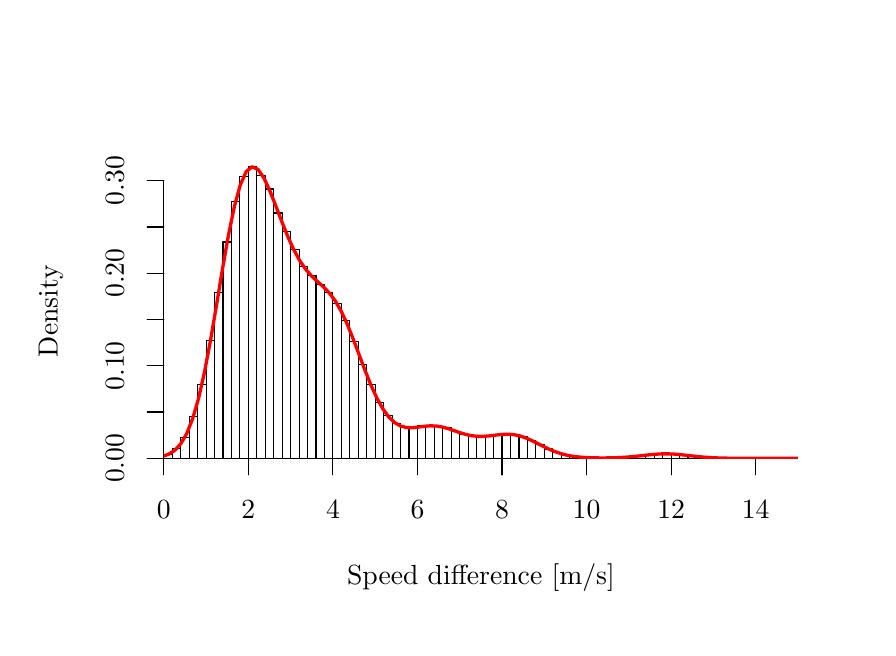
\begin{tikzpicture}[x=1pt,y=1pt]
\definecolor{fillColor}{RGB}{255,255,255}
\path[use as bounding box,fill=fillColor,fill opacity=0.00] (0,0) rectangle (303.53,216.81);
\begin{scope}
\path[clip] (  0.00,  0.00) rectangle (303.53,216.81);
\definecolor{drawColor}{RGB}{0,0,0}

\node[text=drawColor,anchor=base,inner sep=0pt, outer sep=0pt, scale=  1.00] at (163.77, 15.60) {Speed difference [m/s]};

\node[text=drawColor,rotate= 90.00,anchor=base,inner sep=0pt, outer sep=0pt, scale=  1.00] at ( 10.80,114.41) {Density};
\end{scope}
\begin{scope}
\path[clip] (  0.00,  0.00) rectangle (303.53,216.81);
\definecolor{drawColor}{RGB}{0,0,0}

\path[draw=drawColor,line width= 0.4pt,line join=round,line cap=round] ( 49.20, 61.20) -- (263.06, 61.20);

\path[draw=drawColor,line width= 0.4pt,line join=round,line cap=round] ( 49.20, 61.20) -- ( 49.20, 55.20);

\path[draw=drawColor,line width= 0.4pt,line join=round,line cap=round] ( 79.75, 61.20) -- ( 79.75, 55.20);

\path[draw=drawColor,line width= 0.4pt,line join=round,line cap=round] (110.30, 61.20) -- (110.30, 55.20);

\path[draw=drawColor,line width= 0.4pt,line join=round,line cap=round] (140.85, 61.20) -- (140.85, 55.20);

\path[draw=drawColor,line width= 0.4pt,line join=round,line cap=round] (171.40, 61.20) -- (171.40, 55.20);

\path[draw=drawColor,line width= 0.4pt,line join=round,line cap=round] (201.96, 61.20) -- (201.96, 55.20);

\path[draw=drawColor,line width= 0.4pt,line join=round,line cap=round] (232.51, 61.20) -- (232.51, 55.20);

\path[draw=drawColor,line width= 0.4pt,line join=round,line cap=round] (263.06, 61.20) -- (263.06, 55.20);

\node[text=drawColor,anchor=base,inner sep=0pt, outer sep=0pt, scale=  1.00] at ( 49.20, 39.60) {0};

\node[text=drawColor,anchor=base,inner sep=0pt, outer sep=0pt, scale=  1.00] at ( 79.75, 39.60) {2};

\node[text=drawColor,anchor=base,inner sep=0pt, outer sep=0pt, scale=  1.00] at (110.30, 39.60) {4};

\node[text=drawColor,anchor=base,inner sep=0pt, outer sep=0pt, scale=  1.00] at (140.85, 39.60) {6};

\node[text=drawColor,anchor=base,inner sep=0pt, outer sep=0pt, scale=  1.00] at (171.40, 39.60) {8};

\node[text=drawColor,anchor=base,inner sep=0pt, outer sep=0pt, scale=  1.00] at (201.96, 39.60) {10};

\node[text=drawColor,anchor=base,inner sep=0pt, outer sep=0pt, scale=  1.00] at (232.51, 39.60) {12};

\node[text=drawColor,anchor=base,inner sep=0pt, outer sep=0pt, scale=  1.00] at (263.06, 39.60) {14};

\path[draw=drawColor,line width= 0.4pt,line join=round,line cap=round] ( 49.20, 61.20) -- ( 49.20,161.51);

\path[draw=drawColor,line width= 0.4pt,line join=round,line cap=round] ( 49.20, 61.20) -- ( 43.20, 61.20);

\path[draw=drawColor,line width= 0.4pt,line join=round,line cap=round] ( 49.20, 77.92) -- ( 43.20, 77.92);

\path[draw=drawColor,line width= 0.4pt,line join=round,line cap=round] ( 49.20, 94.64) -- ( 43.20, 94.64);

\path[draw=drawColor,line width= 0.4pt,line join=round,line cap=round] ( 49.20,111.36) -- ( 43.20,111.36);

\path[draw=drawColor,line width= 0.4pt,line join=round,line cap=round] ( 49.20,128.08) -- ( 43.20,128.08);

\path[draw=drawColor,line width= 0.4pt,line join=round,line cap=round] ( 49.20,144.79) -- ( 43.20,144.79);

\path[draw=drawColor,line width= 0.4pt,line join=round,line cap=round] ( 49.20,161.51) -- ( 43.20,161.51);

\node[text=drawColor,rotate= 90.00,anchor=base,inner sep=0pt, outer sep=0pt, scale=  1.00] at ( 34.80, 61.20) {0.00};

\node[text=drawColor,rotate= 90.00,anchor=base,inner sep=0pt, outer sep=0pt, scale=  1.00] at ( 34.80, 94.64) {0.10};

\node[text=drawColor,rotate= 90.00,anchor=base,inner sep=0pt, outer sep=0pt, scale=  1.00] at ( 34.80,128.08) {0.20};

\node[text=drawColor,rotate= 90.00,anchor=base,inner sep=0pt, outer sep=0pt, scale=  1.00] at ( 34.80,161.51) {0.30};
\end{scope}
\begin{scope}
\path[clip] ( 49.20, 61.20) rectangle (278.33,167.61);
\definecolor{drawColor}{RGB}{0,0,0}

\path[draw=drawColor,line width= 0.4pt,line join=round,line cap=round] ( 30.87, 61.20) rectangle ( 33.92, 61.20);

\path[draw=drawColor,line width= 0.4pt,line join=round,line cap=round] ( 33.92, 61.20) rectangle ( 36.98, 61.20);

\path[draw=drawColor,line width= 0.4pt,line join=round,line cap=round] ( 36.98, 61.20) rectangle ( 40.03, 61.21);

\path[draw=drawColor,line width= 0.4pt,line join=round,line cap=round] ( 40.03, 61.20) rectangle ( 43.09, 61.24);

\path[draw=drawColor,line width= 0.4pt,line join=round,line cap=round] ( 43.09, 61.20) rectangle ( 46.14, 61.35);

\path[draw=drawColor,line width= 0.4pt,line join=round,line cap=round] ( 46.14, 61.20) rectangle ( 49.20, 61.74);

\path[draw=drawColor,line width= 0.4pt,line join=round,line cap=round] ( 49.20, 61.20) rectangle ( 52.26, 62.64);

\path[draw=drawColor,line width= 0.4pt,line join=round,line cap=round] ( 52.26, 61.20) rectangle ( 55.31, 64.76);

\path[draw=drawColor,line width= 0.4pt,line join=round,line cap=round] ( 55.31, 61.20) rectangle ( 58.37, 68.82);

\path[draw=drawColor,line width= 0.4pt,line join=round,line cap=round] ( 58.37, 61.20) rectangle ( 61.42, 76.40);

\path[draw=drawColor,line width= 0.4pt,line join=round,line cap=round] ( 61.42, 61.20) rectangle ( 64.48, 88.02);

\path[draw=drawColor,line width= 0.4pt,line join=round,line cap=round] ( 64.48, 61.20) rectangle ( 67.53,103.69);

\path[draw=drawColor,line width= 0.4pt,line join=round,line cap=round] ( 67.53, 61.20) rectangle ( 70.59,121.23);

\path[draw=drawColor,line width= 0.4pt,line join=round,line cap=round] ( 70.59, 61.20) rectangle ( 73.64,139.38);

\path[draw=drawColor,line width= 0.4pt,line join=round,line cap=round] ( 73.64, 61.20) rectangle ( 76.70,153.96);

\path[draw=drawColor,line width= 0.4pt,line join=round,line cap=round] ( 76.70, 61.20) rectangle ( 79.75,163.11);

\path[draw=drawColor,line width= 0.4pt,line join=round,line cap=round] ( 79.75, 61.20) rectangle ( 82.81,166.79);

\path[draw=drawColor,line width= 0.4pt,line join=round,line cap=round] ( 82.81, 61.20) rectangle ( 85.86,163.49);

\path[draw=drawColor,line width= 0.4pt,line join=round,line cap=round] ( 85.86, 61.20) rectangle ( 88.92,158.50);

\path[draw=drawColor,line width= 0.4pt,line join=round,line cap=round] ( 88.92, 61.20) rectangle ( 91.97,149.83);

\path[draw=drawColor,line width= 0.4pt,line join=round,line cap=round] ( 91.97, 61.20) rectangle ( 95.03,143.03);

\path[draw=drawColor,line width= 0.4pt,line join=round,line cap=round] ( 95.03, 61.20) rectangle ( 98.08,136.77);

\path[draw=drawColor,line width= 0.4pt,line join=round,line cap=round] ( 98.08, 61.20) rectangle (101.14,130.54);

\path[draw=drawColor,line width= 0.4pt,line join=round,line cap=round] (101.14, 61.20) rectangle (104.19,127.19);

\path[draw=drawColor,line width= 0.4pt,line join=round,line cap=round] (104.19, 61.20) rectangle (107.25,124.15);

\path[draw=drawColor,line width= 0.4pt,line join=round,line cap=round] (107.25, 61.20) rectangle (110.30,121.00);

\path[draw=drawColor,line width= 0.4pt,line join=round,line cap=round] (110.30, 61.20) rectangle (113.36,116.99);

\path[draw=drawColor,line width= 0.4pt,line join=round,line cap=round] (113.36, 61.20) rectangle (116.41,110.96);

\path[draw=drawColor,line width= 0.4pt,line join=round,line cap=round] (116.41, 61.20) rectangle (119.47,103.30);

\path[draw=drawColor,line width= 0.4pt,line join=round,line cap=round] (119.47, 61.20) rectangle (122.52, 95.00);

\path[draw=drawColor,line width= 0.4pt,line join=round,line cap=round] (122.52, 61.20) rectangle (125.58, 87.79);

\path[draw=drawColor,line width= 0.4pt,line join=round,line cap=round] (125.58, 61.20) rectangle (128.63, 81.28);

\path[draw=drawColor,line width= 0.4pt,line join=round,line cap=round] (128.63, 61.20) rectangle (131.69, 76.79);

\path[draw=drawColor,line width= 0.4pt,line join=round,line cap=round] (131.69, 61.20) rectangle (134.74, 73.65);

\path[draw=drawColor,line width= 0.4pt,line join=round,line cap=round] (134.74, 61.20) rectangle (137.80, 72.61);

\path[draw=drawColor,line width= 0.4pt,line join=round,line cap=round] (137.80, 61.20) rectangle (140.85, 72.02);

\path[draw=drawColor,line width= 0.4pt,line join=round,line cap=round] (140.85, 61.20) rectangle (143.91, 72.92);

\path[draw=drawColor,line width= 0.4pt,line join=round,line cap=round] (143.91, 61.20) rectangle (146.96, 73.02);

\path[draw=drawColor,line width= 0.4pt,line join=round,line cap=round] (146.96, 61.20) rectangle (150.02, 72.71);

\path[draw=drawColor,line width= 0.4pt,line join=round,line cap=round] (150.02, 61.20) rectangle (153.07, 72.15);

\path[draw=drawColor,line width= 0.4pt,line join=round,line cap=round] (153.07, 61.20) rectangle (156.13, 70.97);

\path[draw=drawColor,line width= 0.4pt,line join=round,line cap=round] (156.13, 61.20) rectangle (159.18, 69.85);

\path[draw=drawColor,line width= 0.4pt,line join=round,line cap=round] (159.18, 61.20) rectangle (162.24, 69.47);

\path[draw=drawColor,line width= 0.4pt,line join=round,line cap=round] (162.24, 61.20) rectangle (165.29, 69.30);

\path[draw=drawColor,line width= 0.4pt,line join=round,line cap=round] (165.29, 61.20) rectangle (168.35, 69.16);

\path[draw=drawColor,line width= 0.4pt,line join=round,line cap=round] (168.35, 61.20) rectangle (171.40, 69.74);

\path[draw=drawColor,line width= 0.4pt,line join=round,line cap=round] (171.40, 61.20) rectangle (174.46, 69.85);

\path[draw=drawColor,line width= 0.4pt,line join=round,line cap=round] (174.46, 61.20) rectangle (177.52, 69.51);

\path[draw=drawColor,line width= 0.4pt,line join=round,line cap=round] (177.52, 61.20) rectangle (180.57, 68.97);

\path[draw=drawColor,line width= 0.4pt,line join=round,line cap=round] (180.57, 61.20) rectangle (183.63, 67.71);

\path[draw=drawColor,line width= 0.4pt,line join=round,line cap=round] (183.63, 61.20) rectangle (186.68, 66.04);

\path[draw=drawColor,line width= 0.4pt,line join=round,line cap=round] (186.68, 61.20) rectangle (189.74, 64.58);

\path[draw=drawColor,line width= 0.4pt,line join=round,line cap=round] (189.74, 61.20) rectangle (192.79, 63.31);

\path[draw=drawColor,line width= 0.4pt,line join=round,line cap=round] (192.79, 61.20) rectangle (195.85, 62.46);

\path[draw=drawColor,line width= 0.4pt,line join=round,line cap=round] (195.85, 61.20) rectangle (198.90, 61.81);

\path[draw=drawColor,line width= 0.4pt,line join=round,line cap=round] (198.90, 61.20) rectangle (201.96, 61.56);

\path[draw=drawColor,line width= 0.4pt,line join=round,line cap=round] (201.96, 61.20) rectangle (205.01, 61.40);

\path[draw=drawColor,line width= 0.4pt,line join=round,line cap=round] (205.01, 61.20) rectangle (208.07, 61.34);

\path[draw=drawColor,line width= 0.4pt,line join=round,line cap=round] (208.07, 61.20) rectangle (211.12, 61.35);

\path[draw=drawColor,line width= 0.4pt,line join=round,line cap=round] (211.12, 61.20) rectangle (214.18, 61.39);

\path[draw=drawColor,line width= 0.4pt,line join=round,line cap=round] (214.18, 61.20) rectangle (217.23, 61.61);

\path[draw=drawColor,line width= 0.4pt,line join=round,line cap=round] (217.23, 61.20) rectangle (220.29, 61.87);

\path[draw=drawColor,line width= 0.4pt,line join=round,line cap=round] (220.29, 61.20) rectangle (223.34, 62.15);

\path[draw=drawColor,line width= 0.4pt,line join=round,line cap=round] (223.34, 61.20) rectangle (226.40, 62.49);

\path[draw=drawColor,line width= 0.4pt,line join=round,line cap=round] (226.40, 61.20) rectangle (229.45, 62.74);

\path[draw=drawColor,line width= 0.4pt,line join=round,line cap=round] (229.45, 61.20) rectangle (232.51, 62.68);

\path[draw=drawColor,line width= 0.4pt,line join=round,line cap=round] (232.51, 61.20) rectangle (235.56, 62.65);

\path[draw=drawColor,line width= 0.4pt,line join=round,line cap=round] (235.56, 61.20) rectangle (238.62, 62.34);

\path[draw=drawColor,line width= 0.4pt,line join=round,line cap=round] (238.62, 61.20) rectangle (241.67, 62.00);

\path[draw=drawColor,line width= 0.4pt,line join=round,line cap=round] (241.67, 61.20) rectangle (244.73, 61.65);

\path[draw=drawColor,line width= 0.4pt,line join=round,line cap=round] (244.73, 61.20) rectangle (247.78, 61.48);

\path[draw=drawColor,line width= 0.4pt,line join=round,line cap=round] (247.78, 61.20) rectangle (250.84, 61.33);

\path[draw=drawColor,line width= 0.4pt,line join=round,line cap=round] (250.84, 61.20) rectangle (253.89, 61.26);

\path[draw=drawColor,line width= 0.4pt,line join=round,line cap=round] (253.89, 61.20) rectangle (256.95, 61.23);

\path[draw=drawColor,line width= 0.4pt,line join=round,line cap=round] (256.95, 61.20) rectangle (260.00, 61.21);

\path[draw=drawColor,line width= 0.4pt,line join=round,line cap=round] (260.00, 61.20) rectangle (263.06, 61.21);

\path[draw=drawColor,line width= 0.4pt,line join=round,line cap=round] (263.06, 61.20) rectangle (266.11, 61.20);

\path[draw=drawColor,line width= 0.4pt,line join=round,line cap=round] (266.11, 61.20) rectangle (269.17, 61.22);

\path[draw=drawColor,line width= 0.4pt,line join=round,line cap=round] (269.17, 61.20) rectangle (272.22, 61.22);

\path[draw=drawColor,line width= 0.4pt,line join=round,line cap=round] (272.22, 61.20) rectangle (275.28, 61.22);

\path[draw=drawColor,line width= 0.4pt,line join=round,line cap=round] (275.28, 61.20) rectangle (278.33, 61.22);

\path[draw=drawColor,line width= 0.4pt,line join=round,line cap=round] (278.33, 61.20) rectangle (281.39, 61.22);

\path[draw=drawColor,line width= 0.4pt,line join=round,line cap=round] (281.39, 61.20) rectangle (284.44, 61.22);

\path[draw=drawColor,line width= 0.4pt,line join=round,line cap=round] (284.44, 61.20) rectangle (287.50, 61.21);

\path[draw=drawColor,line width= 0.4pt,line join=round,line cap=round] (287.50, 61.20) rectangle (290.55, 61.22);

\path[draw=drawColor,line width= 0.4pt,line join=round,line cap=round] (290.55, 61.20) rectangle (293.61, 61.21);

\path[draw=drawColor,line width= 0.4pt,line join=round,line cap=round] (293.61, 61.20) rectangle (296.66, 61.21);

\path[draw=drawColor,line width= 0.4pt,line join=round,line cap=round] (296.66, 61.20) rectangle (299.72, 61.20);

\path[draw=drawColor,line width= 0.4pt,line join=round,line cap=round] (299.72, 61.20) rectangle (302.77, 61.20);

\path[draw=drawColor,line width= 0.4pt,line join=round,line cap=round] (302.77, 61.20) rectangle (305.83, 61.20);
\definecolor{drawColor}{RGB}{255,0,0}

\path[draw=drawColor,line width= 1.2pt,line join=round,line cap=round] (  0.00, 61.20) --
	(  1.66, 61.20) --
	(  3.80, 61.20) --
	(  5.95, 61.20) --
	(  8.10, 61.20) --
	( 10.24, 61.20) --
	( 12.39, 61.20) --
	( 14.54, 61.20) --
	( 16.69, 61.20) --
	( 18.83, 61.20) --
	( 20.98, 61.20) --
	( 23.13, 61.20) --
	( 25.27, 61.20) --
	( 27.42, 61.20) --
	( 29.57, 61.20) --
	( 31.72, 61.20) --
	( 33.86, 61.20) --
	( 36.01, 61.20) --
	( 38.16, 61.21) --
	( 40.30, 61.22) --
	( 42.45, 61.26) --
	( 44.60, 61.35) --
	( 46.75, 61.55) --
	( 48.89, 61.95) --
	( 51.04, 62.73) --
	( 53.19, 64.12) --
	( 55.33, 66.46) --
	( 57.48, 70.14) --
	( 59.63, 75.55) --
	( 61.78, 82.97) --
	( 63.92, 92.48) --
	( 66.07,103.84) --
	( 68.22,116.44) --
	( 70.36,129.39) --
	( 72.51,141.61) --
	( 74.66,152.06) --
	( 76.81,159.94) --
	( 78.95,164.78) --
	( 81.10,166.56) --
	( 83.25,165.58) --
	( 85.40,162.42) --
	( 87.54,157.78) --
	( 89.69,152.34) --
	( 91.84,146.71) --
	( 93.98,141.36) --
	( 96.13,136.63) --
	( 98.28,132.68) --
	(100.43,129.54) --
	(102.57,127.09) --
	(104.72,125.08) --
	(106.87,123.15) --
	(109.01,120.92) --
	(111.16,118.04) --
	(113.31,114.31) --
	(115.46,109.70) --
	(117.60,104.38) --
	(119.75, 98.68) --
	(121.90, 92.97) --
	(124.04, 87.63) --
	(126.19, 82.94) --
	(128.34, 79.08) --
	(130.49, 76.13) --
	(132.63, 74.08) --
	(134.78, 72.85) --
	(136.93, 72.31) --
	(139.07, 72.25) --
	(141.22, 72.48) --
	(143.37, 72.77) --
	(145.52, 72.94) --
	(147.66, 72.86) --
	(149.81, 72.51) --
	(151.96, 71.92) --
	(154.10, 71.19) --
	(156.25, 70.44) --
	(158.40, 69.80) --
	(160.55, 69.35) --
	(162.69, 69.13) --
	(164.84, 69.14) --
	(166.99, 69.32) --
	(169.13, 69.59) --
	(171.28, 69.82) --
	(173.43, 69.91) --
	(175.58, 69.76) --
	(177.72, 69.33) --
	(179.87, 68.62) --
	(182.02, 67.68) --
	(184.17, 66.61) --
	(186.31, 65.51) --
	(188.46, 64.48) --
	(190.61, 63.59) --
	(192.75, 62.86) --
	(194.90, 62.31) --
	(197.05, 61.92) --
	(199.20, 61.66) --
	(201.34, 61.49) --
	(203.49, 61.40) --
	(205.64, 61.35) --
	(207.78, 61.33) --
	(209.93, 61.35) --
	(212.08, 61.39) --
	(214.23, 61.48) --
	(216.37, 61.62) --
	(218.52, 61.80) --
	(220.67, 62.02) --
	(222.81, 62.27) --
	(224.96, 62.50) --
	(227.11, 62.69) --
	(229.26, 62.80) --
	(231.40, 62.81) --
	(233.55, 62.72) --
	(235.70, 62.54) --
	(237.84, 62.31) --
	(239.99, 62.06) --
	(242.14, 61.83) --
	(244.29, 61.63) --
	(246.43, 61.48) --
	(248.58, 61.37) --
	(250.73, 61.29) --
	(252.87, 61.25) --
	(255.02, 61.23) --
	(257.17, 61.21) --
	(259.32, 61.21) --
	(261.46, 61.21) --
	(263.61, 61.21) --
	(265.76, 61.21) --
	(267.90, 61.21) --
	(270.05, 61.21) --
	(272.20, 61.21) --
	(274.35, 61.22) --
	(276.49, 61.22) --
	(278.64, 61.22) --
	(280.79, 61.22) --
	(282.94, 61.22) --
	(285.08, 61.21) --
	(287.23, 61.21) --
	(289.38, 61.21) --
	(291.52, 61.21) --
	(293.67, 61.20) --
	(295.82, 61.20) --
	(297.97, 61.20) --
	(300.11, 61.20) --
	(302.26, 61.20) --
	(303.53, 61.20);
\end{scope}
\end{tikzpicture}

	\caption{The histogram shows the result of the conditional sampling according to \cref{alg:conditional simple}. The red line represents the true \ac{pdf}.}
	\label{fig:conditional simple}
\end{figure}

\begin{figure}
	\centering
	% Created by tikzDevice version 0.12.3 on 2021-02-01 12:21:50
% !TEX encoding = UTF-8 Unicode
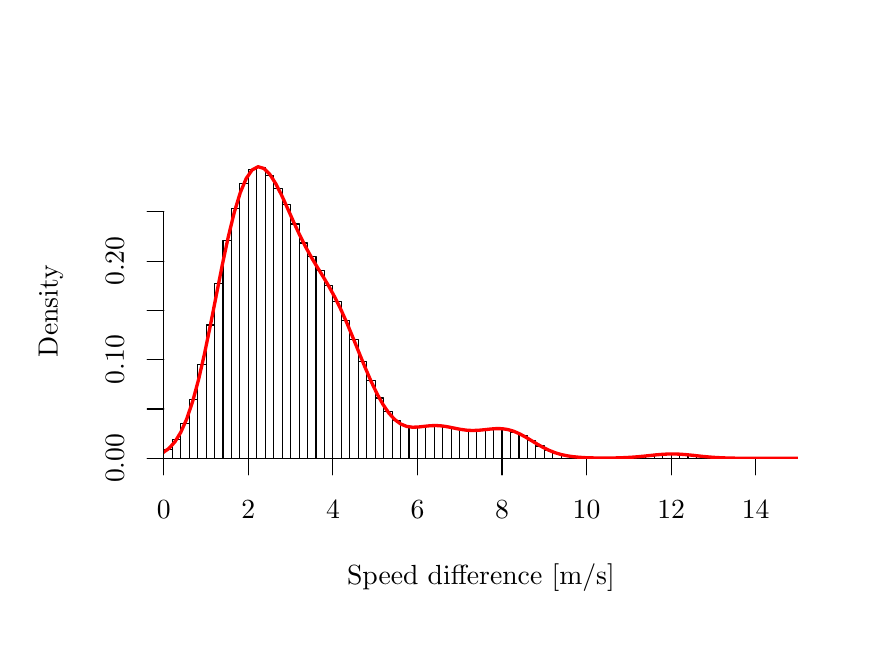
\begin{tikzpicture}[x=1pt,y=1pt]
\definecolor{fillColor}{RGB}{255,255,255}
\path[use as bounding box,fill=fillColor,fill opacity=0.00] (0,0) rectangle (303.53,216.81);
\begin{scope}
\path[clip] (  0.00,  0.00) rectangle (303.53,216.81);
\definecolor{drawColor}{RGB}{0,0,0}

\node[text=drawColor,anchor=base,inner sep=0pt, outer sep=0pt, scale=  1.00] at (163.77, 15.60) {Speed difference [m/s]};

\node[text=drawColor,rotate= 90.00,anchor=base,inner sep=0pt, outer sep=0pt, scale=  1.00] at ( 10.80,114.41) {Density};
\end{scope}
\begin{scope}
\path[clip] (  0.00,  0.00) rectangle (303.53,216.81);
\definecolor{drawColor}{RGB}{0,0,0}

\path[draw=drawColor,line width= 0.4pt,line join=round,line cap=round] ( 49.20, 61.20) -- (263.06, 61.20);

\path[draw=drawColor,line width= 0.4pt,line join=round,line cap=round] ( 49.20, 61.20) -- ( 49.20, 55.20);

\path[draw=drawColor,line width= 0.4pt,line join=round,line cap=round] ( 79.75, 61.20) -- ( 79.75, 55.20);

\path[draw=drawColor,line width= 0.4pt,line join=round,line cap=round] (110.30, 61.20) -- (110.30, 55.20);

\path[draw=drawColor,line width= 0.4pt,line join=round,line cap=round] (140.85, 61.20) -- (140.85, 55.20);

\path[draw=drawColor,line width= 0.4pt,line join=round,line cap=round] (171.40, 61.20) -- (171.40, 55.20);

\path[draw=drawColor,line width= 0.4pt,line join=round,line cap=round] (201.96, 61.20) -- (201.96, 55.20);

\path[draw=drawColor,line width= 0.4pt,line join=round,line cap=round] (232.51, 61.20) -- (232.51, 55.20);

\path[draw=drawColor,line width= 0.4pt,line join=round,line cap=round] (263.06, 61.20) -- (263.06, 55.20);

\node[text=drawColor,anchor=base,inner sep=0pt, outer sep=0pt, scale=  1.00] at ( 49.20, 39.60) {0};

\node[text=drawColor,anchor=base,inner sep=0pt, outer sep=0pt, scale=  1.00] at ( 79.75, 39.60) {2};

\node[text=drawColor,anchor=base,inner sep=0pt, outer sep=0pt, scale=  1.00] at (110.30, 39.60) {4};

\node[text=drawColor,anchor=base,inner sep=0pt, outer sep=0pt, scale=  1.00] at (140.85, 39.60) {6};

\node[text=drawColor,anchor=base,inner sep=0pt, outer sep=0pt, scale=  1.00] at (171.40, 39.60) {8};

\node[text=drawColor,anchor=base,inner sep=0pt, outer sep=0pt, scale=  1.00] at (201.96, 39.60) {10};

\node[text=drawColor,anchor=base,inner sep=0pt, outer sep=0pt, scale=  1.00] at (232.51, 39.60) {12};

\node[text=drawColor,anchor=base,inner sep=0pt, outer sep=0pt, scale=  1.00] at (263.06, 39.60) {14};

\path[draw=drawColor,line width= 0.4pt,line join=round,line cap=round] ( 49.20, 61.20) -- ( 49.20,150.23);

\path[draw=drawColor,line width= 0.4pt,line join=round,line cap=round] ( 49.20, 61.20) -- ( 43.20, 61.20);

\path[draw=drawColor,line width= 0.4pt,line join=round,line cap=round] ( 49.20, 79.01) -- ( 43.20, 79.01);

\path[draw=drawColor,line width= 0.4pt,line join=round,line cap=round] ( 49.20, 96.81) -- ( 43.20, 96.81);

\path[draw=drawColor,line width= 0.4pt,line join=round,line cap=round] ( 49.20,114.62) -- ( 43.20,114.62);

\path[draw=drawColor,line width= 0.4pt,line join=round,line cap=round] ( 49.20,132.42) -- ( 43.20,132.42);

\path[draw=drawColor,line width= 0.4pt,line join=round,line cap=round] ( 49.20,150.23) -- ( 43.20,150.23);

\node[text=drawColor,rotate= 90.00,anchor=base,inner sep=0pt, outer sep=0pt, scale=  1.00] at ( 34.80, 61.20) {0.00};

\node[text=drawColor,rotate= 90.00,anchor=base,inner sep=0pt, outer sep=0pt, scale=  1.00] at ( 34.80, 96.81) {0.10};

\node[text=drawColor,rotate= 90.00,anchor=base,inner sep=0pt, outer sep=0pt, scale=  1.00] at ( 34.80,132.42) {0.20};
\end{scope}
\begin{scope}
\path[clip] ( 49.20, 61.20) rectangle (278.33,167.61);
\definecolor{drawColor}{RGB}{0,0,0}

\path[draw=drawColor,line width= 0.4pt,line join=round,line cap=round] ( -2.74, 61.20) rectangle (  0.32, 61.20);

\path[draw=drawColor,line width= 0.4pt,line join=round,line cap=round] (  0.32, 61.20) rectangle (  3.37, 61.20);

\path[draw=drawColor,line width= 0.4pt,line join=round,line cap=round] (  3.37, 61.20) rectangle (  6.43, 61.20);

\path[draw=drawColor,line width= 0.4pt,line join=round,line cap=round] (  6.43, 61.20) rectangle (  9.48, 61.20);

\path[draw=drawColor,line width= 0.4pt,line join=round,line cap=round] (  9.48, 61.20) rectangle ( 12.54, 61.20);

\path[draw=drawColor,line width= 0.4pt,line join=round,line cap=round] ( 12.54, 61.20) rectangle ( 15.59, 61.20);

\path[draw=drawColor,line width= 0.4pt,line join=round,line cap=round] ( 15.59, 61.20) rectangle ( 18.65, 61.20);

\path[draw=drawColor,line width= 0.4pt,line join=round,line cap=round] ( 18.65, 61.20) rectangle ( 21.70, 61.20);

\path[draw=drawColor,line width= 0.4pt,line join=round,line cap=round] ( 21.70, 61.20) rectangle ( 24.76, 61.20);

\path[draw=drawColor,line width= 0.4pt,line join=round,line cap=round] ( 24.76, 61.20) rectangle ( 27.81, 61.20);

\path[draw=drawColor,line width= 0.4pt,line join=round,line cap=round] ( 27.81, 61.20) rectangle ( 30.87, 61.20);

\path[draw=drawColor,line width= 0.4pt,line join=round,line cap=round] ( 30.87, 61.20) rectangle ( 33.92, 61.21);

\path[draw=drawColor,line width= 0.4pt,line join=round,line cap=round] ( 33.92, 61.20) rectangle ( 36.98, 61.22);

\path[draw=drawColor,line width= 0.4pt,line join=round,line cap=round] ( 36.98, 61.20) rectangle ( 40.03, 61.28);

\path[draw=drawColor,line width= 0.4pt,line join=round,line cap=round] ( 40.03, 61.20) rectangle ( 43.09, 61.42);

\path[draw=drawColor,line width= 0.4pt,line join=round,line cap=round] ( 43.09, 61.20) rectangle ( 46.14, 61.79);

\path[draw=drawColor,line width= 0.4pt,line join=round,line cap=round] ( 46.14, 61.20) rectangle ( 49.20, 62.58);

\path[draw=drawColor,line width= 0.4pt,line join=round,line cap=round] ( 49.20, 61.20) rectangle ( 52.26, 64.52);

\path[draw=drawColor,line width= 0.4pt,line join=round,line cap=round] ( 52.26, 61.20) rectangle ( 55.31, 67.92);

\path[draw=drawColor,line width= 0.4pt,line join=round,line cap=round] ( 55.31, 61.20) rectangle ( 58.37, 73.86);

\path[draw=drawColor,line width= 0.4pt,line join=round,line cap=round] ( 58.37, 61.20) rectangle ( 61.42, 82.52);

\path[draw=drawColor,line width= 0.4pt,line join=round,line cap=round] ( 61.42, 61.20) rectangle ( 64.48, 94.94);

\path[draw=drawColor,line width= 0.4pt,line join=round,line cap=round] ( 64.48, 61.20) rectangle ( 67.53,109.36);

\path[draw=drawColor,line width= 0.4pt,line join=round,line cap=round] ( 67.53, 61.20) rectangle ( 70.59,124.31);

\path[draw=drawColor,line width= 0.4pt,line join=round,line cap=round] ( 70.59, 61.20) rectangle ( 73.64,140.00);

\path[draw=drawColor,line width= 0.4pt,line join=round,line cap=round] ( 73.64, 61.20) rectangle ( 76.70,151.43);

\path[draw=drawColor,line width= 0.4pt,line join=round,line cap=round] ( 76.70, 61.20) rectangle ( 79.75,160.44);

\path[draw=drawColor,line width= 0.4pt,line join=round,line cap=round] ( 79.75, 61.20) rectangle ( 82.81,165.63);

\path[draw=drawColor,line width= 0.4pt,line join=round,line cap=round] ( 82.81, 61.20) rectangle ( 85.86,166.14);

\path[draw=drawColor,line width= 0.4pt,line join=round,line cap=round] ( 85.86, 61.20) rectangle ( 88.92,163.35);

\path[draw=drawColor,line width= 0.4pt,line join=round,line cap=round] ( 88.92, 61.20) rectangle ( 91.97,158.64);

\path[draw=drawColor,line width= 0.4pt,line join=round,line cap=round] ( 91.97, 61.20) rectangle ( 95.03,152.76);

\path[draw=drawColor,line width= 0.4pt,line join=round,line cap=round] ( 95.03, 61.20) rectangle ( 98.08,145.88);

\path[draw=drawColor,line width= 0.4pt,line join=round,line cap=round] ( 98.08, 61.20) rectangle (101.14,138.99);

\path[draw=drawColor,line width= 0.4pt,line join=round,line cap=round] (101.14, 61.20) rectangle (104.19,134.01);

\path[draw=drawColor,line width= 0.4pt,line join=round,line cap=round] (104.19, 61.20) rectangle (107.25,128.93);

\path[draw=drawColor,line width= 0.4pt,line join=round,line cap=round] (107.25, 61.20) rectangle (110.30,123.61);

\path[draw=drawColor,line width= 0.4pt,line join=round,line cap=round] (110.30, 61.20) rectangle (113.36,117.73);

\path[draw=drawColor,line width= 0.4pt,line join=round,line cap=round] (113.36, 61.20) rectangle (116.41,111.10);

\path[draw=drawColor,line width= 0.4pt,line join=round,line cap=round] (116.41, 61.20) rectangle (119.47,104.05);

\path[draw=drawColor,line width= 0.4pt,line join=round,line cap=round] (119.47, 61.20) rectangle (122.52, 96.15);

\path[draw=drawColor,line width= 0.4pt,line join=round,line cap=round] (122.52, 61.20) rectangle (125.58, 89.22);

\path[draw=drawColor,line width= 0.4pt,line join=round,line cap=round] (125.58, 61.20) rectangle (128.63, 83.01);

\path[draw=drawColor,line width= 0.4pt,line join=round,line cap=round] (128.63, 61.20) rectangle (131.69, 78.15);

\path[draw=drawColor,line width= 0.4pt,line join=round,line cap=round] (131.69, 61.20) rectangle (134.74, 74.72);

\path[draw=drawColor,line width= 0.4pt,line join=round,line cap=round] (134.74, 61.20) rectangle (137.80, 73.02);

\path[draw=drawColor,line width= 0.4pt,line join=round,line cap=round] (137.80, 61.20) rectangle (140.85, 72.35);

\path[draw=drawColor,line width= 0.4pt,line join=round,line cap=round] (140.85, 61.20) rectangle (143.91, 72.44);

\path[draw=drawColor,line width= 0.4pt,line join=round,line cap=round] (143.91, 61.20) rectangle (146.96, 72.89);

\path[draw=drawColor,line width= 0.4pt,line join=round,line cap=round] (146.96, 61.20) rectangle (150.02, 73.10);

\path[draw=drawColor,line width= 0.4pt,line join=round,line cap=round] (150.02, 61.20) rectangle (153.07, 72.71);

\path[draw=drawColor,line width= 0.4pt,line join=round,line cap=round] (153.07, 61.20) rectangle (156.13, 71.89);

\path[draw=drawColor,line width= 0.4pt,line join=round,line cap=round] (156.13, 61.20) rectangle (159.18, 71.57);

\path[draw=drawColor,line width= 0.4pt,line join=round,line cap=round] (159.18, 61.20) rectangle (162.24, 71.58);

\path[draw=drawColor,line width= 0.4pt,line join=round,line cap=round] (162.24, 61.20) rectangle (165.29, 71.39);

\path[draw=drawColor,line width= 0.4pt,line join=round,line cap=round] (165.29, 61.20) rectangle (168.35, 71.85);

\path[draw=drawColor,line width= 0.4pt,line join=round,line cap=round] (168.35, 61.20) rectangle (171.40, 71.77);

\path[draw=drawColor,line width= 0.4pt,line join=round,line cap=round] (171.40, 61.20) rectangle (174.46, 71.67);

\path[draw=drawColor,line width= 0.4pt,line join=round,line cap=round] (174.46, 61.20) rectangle (177.52, 70.65);

\path[draw=drawColor,line width= 0.4pt,line join=round,line cap=round] (177.52, 61.20) rectangle (180.57, 69.29);

\path[draw=drawColor,line width= 0.4pt,line join=round,line cap=round] (180.57, 61.20) rectangle (183.63, 67.55);

\path[draw=drawColor,line width= 0.4pt,line join=round,line cap=round] (183.63, 61.20) rectangle (186.68, 65.66);

\path[draw=drawColor,line width= 0.4pt,line join=round,line cap=round] (186.68, 61.20) rectangle (189.74, 64.17);

\path[draw=drawColor,line width= 0.4pt,line join=round,line cap=round] (189.74, 61.20) rectangle (192.79, 63.03);

\path[draw=drawColor,line width= 0.4pt,line join=round,line cap=round] (192.79, 61.20) rectangle (195.85, 62.30);

\path[draw=drawColor,line width= 0.4pt,line join=round,line cap=round] (195.85, 61.20) rectangle (198.90, 61.76);

\path[draw=drawColor,line width= 0.4pt,line join=round,line cap=round] (198.90, 61.20) rectangle (201.96, 61.47);

\path[draw=drawColor,line width= 0.4pt,line join=round,line cap=round] (201.96, 61.20) rectangle (205.01, 61.36);

\path[draw=drawColor,line width= 0.4pt,line join=round,line cap=round] (205.01, 61.20) rectangle (208.07, 61.30);

\path[draw=drawColor,line width= 0.4pt,line join=round,line cap=round] (208.07, 61.20) rectangle (211.12, 61.29);

\path[draw=drawColor,line width= 0.4pt,line join=round,line cap=round] (211.12, 61.20) rectangle (214.18, 61.35);

\path[draw=drawColor,line width= 0.4pt,line join=round,line cap=round] (214.18, 61.20) rectangle (217.23, 61.43);

\path[draw=drawColor,line width= 0.4pt,line join=round,line cap=round] (217.23, 61.20) rectangle (220.29, 61.61);

\path[draw=drawColor,line width= 0.4pt,line join=round,line cap=round] (220.29, 61.20) rectangle (223.34, 61.90);

\path[draw=drawColor,line width= 0.4pt,line join=round,line cap=round] (223.34, 61.20) rectangle (226.40, 62.21);

\path[draw=drawColor,line width= 0.4pt,line join=round,line cap=round] (226.40, 61.20) rectangle (229.45, 62.54);

\path[draw=drawColor,line width= 0.4pt,line join=round,line cap=round] (229.45, 61.20) rectangle (232.51, 62.71);

\path[draw=drawColor,line width= 0.4pt,line join=round,line cap=round] (232.51, 61.20) rectangle (235.56, 62.84);

\path[draw=drawColor,line width= 0.4pt,line join=round,line cap=round] (235.56, 61.20) rectangle (238.62, 62.64);

\path[draw=drawColor,line width= 0.4pt,line join=round,line cap=round] (238.62, 61.20) rectangle (241.67, 62.34);

\path[draw=drawColor,line width= 0.4pt,line join=round,line cap=round] (241.67, 61.20) rectangle (244.73, 62.00);

\path[draw=drawColor,line width= 0.4pt,line join=round,line cap=round] (244.73, 61.20) rectangle (247.78, 61.67);

\path[draw=drawColor,line width= 0.4pt,line join=round,line cap=round] (247.78, 61.20) rectangle (250.84, 61.42);

\path[draw=drawColor,line width= 0.4pt,line join=round,line cap=round] (250.84, 61.20) rectangle (253.89, 61.32);

\path[draw=drawColor,line width= 0.4pt,line join=round,line cap=round] (253.89, 61.20) rectangle (256.95, 61.27);

\path[draw=drawColor,line width= 0.4pt,line join=round,line cap=round] (256.95, 61.20) rectangle (260.00, 61.22);

\path[draw=drawColor,line width= 0.4pt,line join=round,line cap=round] (260.00, 61.20) rectangle (263.06, 61.21);

\path[draw=drawColor,line width= 0.4pt,line join=round,line cap=round] (263.06, 61.20) rectangle (266.11, 61.21);

\path[draw=drawColor,line width= 0.4pt,line join=round,line cap=round] (266.11, 61.20) rectangle (269.17, 61.21);

\path[draw=drawColor,line width= 0.4pt,line join=round,line cap=round] (269.17, 61.20) rectangle (272.22, 61.20);

\path[draw=drawColor,line width= 0.4pt,line join=round,line cap=round] (272.22, 61.20) rectangle (275.28, 61.22);

\path[draw=drawColor,line width= 0.4pt,line join=round,line cap=round] (275.28, 61.20) rectangle (278.33, 61.23);

\path[draw=drawColor,line width= 0.4pt,line join=round,line cap=round] (278.33, 61.20) rectangle (281.39, 61.25);

\path[draw=drawColor,line width= 0.4pt,line join=round,line cap=round] (281.39, 61.20) rectangle (284.44, 61.22);

\path[draw=drawColor,line width= 0.4pt,line join=round,line cap=round] (284.44, 61.20) rectangle (287.50, 61.24);

\path[draw=drawColor,line width= 0.4pt,line join=round,line cap=round] (287.50, 61.20) rectangle (290.55, 61.22);

\path[draw=drawColor,line width= 0.4pt,line join=round,line cap=round] (290.55, 61.20) rectangle (293.61, 61.22);

\path[draw=drawColor,line width= 0.4pt,line join=round,line cap=round] (293.61, 61.20) rectangle (296.66, 61.21);

\path[draw=drawColor,line width= 0.4pt,line join=round,line cap=round] (296.66, 61.20) rectangle (299.72, 61.20);

\path[draw=drawColor,line width= 0.4pt,line join=round,line cap=round] (299.72, 61.20) rectangle (302.77, 61.20);

\path[draw=drawColor,line width= 0.4pt,line join=round,line cap=round] (302.77, 61.20) rectangle (305.83, 61.20);
\definecolor{drawColor}{RGB}{255,0,0}

\path[draw=drawColor,line width= 1.2pt,line join=round,line cap=round] (  0.00, 61.20) --
	(  1.66, 61.20) --
	(  3.80, 61.20) --
	(  5.95, 61.20) --
	(  8.10, 61.20) --
	( 10.24, 61.20) --
	( 12.39, 61.20) --
	( 14.54, 61.20) --
	( 16.69, 61.20) --
	( 18.83, 61.20) --
	( 20.98, 61.20) --
	( 23.13, 61.20) --
	( 25.27, 61.20) --
	( 27.42, 61.20) --
	( 29.57, 61.20) --
	( 31.72, 61.20) --
	( 33.86, 61.21) --
	( 36.01, 61.23) --
	( 38.16, 61.26) --
	( 40.30, 61.34) --
	( 42.45, 61.49) --
	( 44.60, 61.78) --
	( 46.75, 62.32) --
	( 48.89, 63.25) --
	( 51.04, 64.77) --
	( 53.19, 67.13) --
	( 55.33, 70.60) --
	( 57.48, 75.44) --
	( 59.63, 81.81) --
	( 61.78, 89.75) --
	( 63.92, 99.10) --
	( 66.07,109.50) --
	( 68.22,120.43) --
	( 70.36,131.25) --
	( 72.51,141.32) --
	( 74.66,150.09) --
	( 76.81,157.16) --
	( 78.95,162.29) --
	( 81.10,165.40) --
	( 83.25,166.56) --
	( 85.40,165.93) --
	( 87.54,163.75) --
	( 89.69,160.36) --
	( 91.84,156.10) --
	( 93.98,151.37) --
	( 96.13,146.54) --
	( 98.28,141.89) --
	(100.43,137.61) --
	(102.57,133.73) --
	(104.72,130.15) --
	(106.87,126.66) --
	(109.01,123.04) --
	(111.16,119.08) --
	(113.31,114.67) --
	(115.46,109.83) --
	(117.60,104.66) --
	(119.75, 99.34) --
	(121.90, 94.10) --
	(124.04, 89.13) --
	(126.19, 84.62) --
	(128.34, 80.73) --
	(130.49, 77.57) --
	(132.63, 75.20) --
	(134.78, 73.61) --
	(136.93, 72.73) --
	(139.07, 72.43) --
	(141.22, 72.51) --
	(143.37, 72.76) --
	(145.52, 72.98) --
	(147.66, 73.04) --
	(149.81, 72.89) --
	(151.96, 72.55) --
	(154.10, 72.11) --
	(156.25, 71.69) --
	(158.40, 71.38) --
	(160.55, 71.25) --
	(162.69, 71.31) --
	(164.84, 71.51) --
	(166.99, 71.75) --
	(169.13, 71.92) --
	(171.28, 71.91) --
	(173.43, 71.61) --
	(175.58, 70.99) --
	(177.72, 70.06) --
	(179.87, 68.90) --
	(182.02, 67.61) --
	(184.17, 66.30) --
	(186.31, 65.10) --
	(188.46, 64.06) --
	(190.61, 63.21) --
	(192.75, 62.57) --
	(194.90, 62.11) --
	(197.05, 61.79) --
	(199.20, 61.58) --
	(201.34, 61.44) --
	(203.49, 61.36) --
	(205.64, 61.32) --
	(207.78, 61.30) --
	(209.93, 61.31) --
	(212.08, 61.33) --
	(214.23, 61.39) --
	(216.37, 61.48) --
	(218.52, 61.61) --
	(220.67, 61.78) --
	(222.81, 61.99) --
	(224.96, 62.22) --
	(227.11, 62.45) --
	(229.26, 62.63) --
	(231.40, 62.75) --
	(233.55, 62.77) --
	(235.70, 62.69) --
	(237.84, 62.53) --
	(239.99, 62.32) --
	(242.14, 62.08) --
	(244.29, 61.85) --
	(246.43, 61.66) --
	(248.58, 61.50) --
	(250.73, 61.39) --
	(252.87, 61.31) --
	(255.02, 61.26) --
	(257.17, 61.23) --
	(259.32, 61.22) --
	(261.46, 61.21) --
	(263.61, 61.21) --
	(265.76, 61.21) --
	(267.90, 61.21) --
	(270.05, 61.21) --
	(272.20, 61.22) --
	(274.35, 61.22) --
	(276.49, 61.23) --
	(278.64, 61.23) --
	(280.79, 61.23) --
	(282.94, 61.23) --
	(285.08, 61.23) --
	(287.23, 61.23) --
	(289.38, 61.23) --
	(291.52, 61.22) --
	(293.67, 61.21) --
	(295.82, 61.21) --
	(297.97, 61.21) --
	(300.11, 61.20) --
	(302.26, 61.20) --
	(303.53, 61.20);
\end{scope}
\end{tikzpicture}

	\caption{The histogram show the result of the conditional sampling according to \cref{alg:conditional hard}. The red line represents the true \ac{pdf}.}
	\label{fig:conditional hard}
\end{figure}



\subsection{Sampling with linear constraints}

In this second example, we want to sample from the \ac{kde} while the generated samples satisfy $\dimensionparta=2$ linear constraints.
More specifically, we want to sample the speed difference, while the average deceleration equals $\SI{1}{\meter\per\second\squared}$ and the start speed equals $\SI{15}{\meter\per\second}$. 
This means that we have
\begin{equation}
	\constraintmatrix = \begin{bmatrix} 1 & 0 & 0 \\ 0 & 1 & 1 \end{bmatrix}, 
	\constraintvector = \begin{bmatrix} 1 \\ 15 \end{bmatrix}.
\end{equation}
The \ac{svd} according to \cref{eq:svd constraint matrix} gives
\begin{equation}
	\svdu = \begin{bmatrix} 0 & 1 \\ 1 & 0 \end{bmatrix},
	\svds = \begin{bmatrix} \sqrt{2} & 0 \\ 0 & 1 \end{bmatrix},
	\svdva = \begin{bmatrix} 0 & 1 \\ \frac{1}{2}\sqrt{2} & 0 \\ \frac{1}{2}\sqrt{2} & 0 \end{bmatrix},
	\svdvb = \begin{bmatrix} 0 \\ -\frac{1}{2}\sqrt{2} \\ \frac{1}{2}\sqrt{2} \end{bmatrix}.
\end{equation}

In \cref{fig:constrained simple,fig:constrained hard}, the result of \cref{alg:constrained simple,alg:constrained hard} is shown, respectively. 
In total $10^6$ samples are generated and shown by the histogram. 
Because the histograms follow the same pattern as the actual density of the speed difference according to the \ac{kde}, it illustrates that the provided algorithms correctly sample from the \ac{kde}. 

\begin{figure}
	\centering
	% Created by tikzDevice version 0.12.3 on 2021-01-29 08:38:57
% !TEX encoding = UTF-8 Unicode
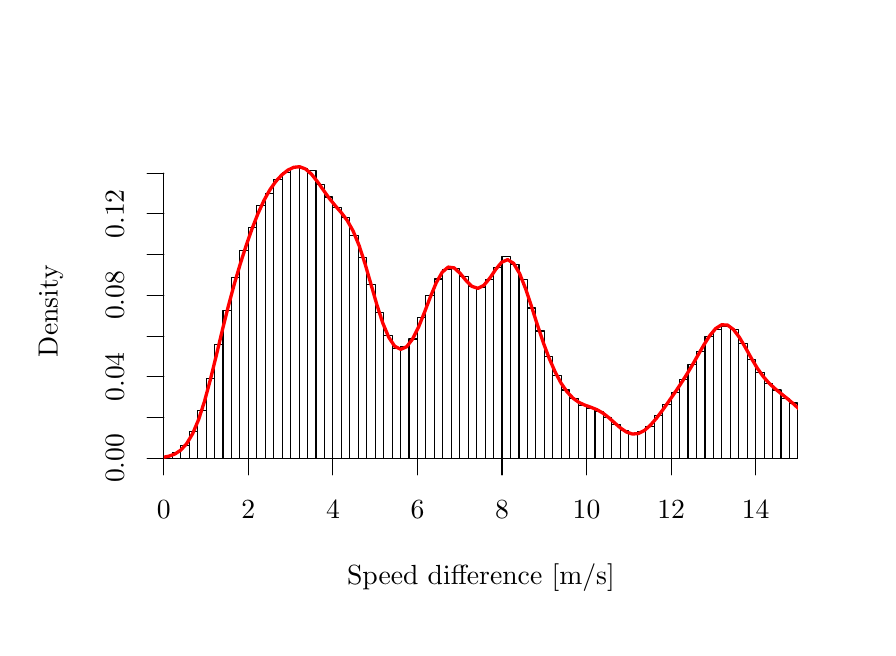
\begin{tikzpicture}[x=1pt,y=1pt]
\definecolor{fillColor}{RGB}{255,255,255}
\path[use as bounding box,fill=fillColor,fill opacity=0.00] (0,0) rectangle (303.53,216.81);
\begin{scope}
\path[clip] (  0.00,  0.00) rectangle (303.53,216.81);
\definecolor{drawColor}{RGB}{0,0,0}

\node[text=drawColor,anchor=base,inner sep=0pt, outer sep=0pt, scale=  1.00] at (163.77, 15.60) {Speed difference [m/s]};

\node[text=drawColor,rotate= 90.00,anchor=base,inner sep=0pt, outer sep=0pt, scale=  1.00] at ( 10.80,114.41) {Density};
\end{scope}
\begin{scope}
\path[clip] (  0.00,  0.00) rectangle (303.53,216.81);
\definecolor{drawColor}{RGB}{0,0,0}

\path[draw=drawColor,line width= 0.4pt,line join=round,line cap=round] ( 49.20, 61.20) -- (263.06, 61.20);

\path[draw=drawColor,line width= 0.4pt,line join=round,line cap=round] ( 49.20, 61.20) -- ( 49.20, 55.20);

\path[draw=drawColor,line width= 0.4pt,line join=round,line cap=round] ( 79.75, 61.20) -- ( 79.75, 55.20);

\path[draw=drawColor,line width= 0.4pt,line join=round,line cap=round] (110.30, 61.20) -- (110.30, 55.20);

\path[draw=drawColor,line width= 0.4pt,line join=round,line cap=round] (140.85, 61.20) -- (140.85, 55.20);

\path[draw=drawColor,line width= 0.4pt,line join=round,line cap=round] (171.40, 61.20) -- (171.40, 55.20);

\path[draw=drawColor,line width= 0.4pt,line join=round,line cap=round] (201.96, 61.20) -- (201.96, 55.20);

\path[draw=drawColor,line width= 0.4pt,line join=round,line cap=round] (232.51, 61.20) -- (232.51, 55.20);

\path[draw=drawColor,line width= 0.4pt,line join=round,line cap=round] (263.06, 61.20) -- (263.06, 55.20);

\node[text=drawColor,anchor=base,inner sep=0pt, outer sep=0pt, scale=  1.00] at ( 49.20, 39.60) {0};

\node[text=drawColor,anchor=base,inner sep=0pt, outer sep=0pt, scale=  1.00] at ( 79.75, 39.60) {2};

\node[text=drawColor,anchor=base,inner sep=0pt, outer sep=0pt, scale=  1.00] at (110.30, 39.60) {4};

\node[text=drawColor,anchor=base,inner sep=0pt, outer sep=0pt, scale=  1.00] at (140.85, 39.60) {6};

\node[text=drawColor,anchor=base,inner sep=0pt, outer sep=0pt, scale=  1.00] at (171.40, 39.60) {8};

\node[text=drawColor,anchor=base,inner sep=0pt, outer sep=0pt, scale=  1.00] at (201.96, 39.60) {10};

\node[text=drawColor,anchor=base,inner sep=0pt, outer sep=0pt, scale=  1.00] at (232.51, 39.60) {12};

\node[text=drawColor,anchor=base,inner sep=0pt, outer sep=0pt, scale=  1.00] at (263.06, 39.60) {14};

\path[draw=drawColor,line width= 0.4pt,line join=round,line cap=round] ( 49.20, 61.20) -- ( 49.20,164.23);

\path[draw=drawColor,line width= 0.4pt,line join=round,line cap=round] ( 49.20, 61.20) -- ( 43.20, 61.20);

\path[draw=drawColor,line width= 0.4pt,line join=round,line cap=round] ( 49.20, 75.92) -- ( 43.20, 75.92);

\path[draw=drawColor,line width= 0.4pt,line join=round,line cap=round] ( 49.20, 90.64) -- ( 43.20, 90.64);

\path[draw=drawColor,line width= 0.4pt,line join=round,line cap=round] ( 49.20,105.36) -- ( 43.20,105.36);

\path[draw=drawColor,line width= 0.4pt,line join=round,line cap=round] ( 49.20,120.07) -- ( 43.20,120.07);

\path[draw=drawColor,line width= 0.4pt,line join=round,line cap=round] ( 49.20,134.79) -- ( 43.20,134.79);

\path[draw=drawColor,line width= 0.4pt,line join=round,line cap=round] ( 49.20,149.51) -- ( 43.20,149.51);

\path[draw=drawColor,line width= 0.4pt,line join=round,line cap=round] ( 49.20,164.23) -- ( 43.20,164.23);

\node[text=drawColor,rotate= 90.00,anchor=base,inner sep=0pt, outer sep=0pt, scale=  1.00] at ( 34.80, 61.20) {0.00};

\node[text=drawColor,rotate= 90.00,anchor=base,inner sep=0pt, outer sep=0pt, scale=  1.00] at ( 34.80, 90.64) {0.04};

\node[text=drawColor,rotate= 90.00,anchor=base,inner sep=0pt, outer sep=0pt, scale=  1.00] at ( 34.80,120.07) {0.08};

\node[text=drawColor,rotate= 90.00,anchor=base,inner sep=0pt, outer sep=0pt, scale=  1.00] at ( 34.80,149.51) {0.12};
\end{scope}
\begin{scope}
\path[clip] ( 49.20, 61.20) rectangle (278.33,167.61);
\definecolor{drawColor}{RGB}{0,0,0}

\path[draw=drawColor,line width= 0.4pt,line join=round,line cap=round] ( 40.03, 61.20) rectangle ( 43.09, 61.23);

\path[draw=drawColor,line width= 0.4pt,line join=round,line cap=round] ( 43.09, 61.20) rectangle ( 46.14, 61.25);

\path[draw=drawColor,line width= 0.4pt,line join=round,line cap=round] ( 46.14, 61.20) rectangle ( 49.20, 61.41);

\path[draw=drawColor,line width= 0.4pt,line join=round,line cap=round] ( 49.20, 61.20) rectangle ( 52.26, 61.87);

\path[draw=drawColor,line width= 0.4pt,line join=round,line cap=round] ( 52.26, 61.20) rectangle ( 55.31, 63.20);

\path[draw=drawColor,line width= 0.4pt,line join=round,line cap=round] ( 55.31, 61.20) rectangle ( 58.37, 65.84);

\path[draw=drawColor,line width= 0.4pt,line join=round,line cap=round] ( 58.37, 61.20) rectangle ( 61.42, 70.86);

\path[draw=drawColor,line width= 0.4pt,line join=round,line cap=round] ( 61.42, 61.20) rectangle ( 64.48, 78.62);

\path[draw=drawColor,line width= 0.4pt,line join=round,line cap=round] ( 64.48, 61.20) rectangle ( 67.53, 89.91);

\path[draw=drawColor,line width= 0.4pt,line join=round,line cap=round] ( 67.53, 61.20) rectangle ( 70.59,102.24);

\path[draw=drawColor,line width= 0.4pt,line join=round,line cap=round] ( 70.59, 61.20) rectangle ( 73.64,114.75);

\path[draw=drawColor,line width= 0.4pt,line join=round,line cap=round] ( 73.64, 61.20) rectangle ( 76.70,126.43);

\path[draw=drawColor,line width= 0.4pt,line join=round,line cap=round] ( 76.70, 61.20) rectangle ( 79.75,136.40);

\path[draw=drawColor,line width= 0.4pt,line join=round,line cap=round] ( 79.75, 61.20) rectangle ( 82.81,144.69);

\path[draw=drawColor,line width= 0.4pt,line join=round,line cap=round] ( 82.81, 61.20) rectangle ( 85.86,152.57);

\path[draw=drawColor,line width= 0.4pt,line join=round,line cap=round] ( 85.86, 61.20) rectangle ( 88.92,156.80);

\path[draw=drawColor,line width= 0.4pt,line join=round,line cap=round] ( 88.92, 61.20) rectangle ( 91.97,162.03);

\path[draw=drawColor,line width= 0.4pt,line join=round,line cap=round] ( 91.97, 61.20) rectangle ( 95.03,164.48);

\path[draw=drawColor,line width= 0.4pt,line join=round,line cap=round] ( 95.03, 61.20) rectangle ( 98.08,166.44);

\path[draw=drawColor,line width= 0.4pt,line join=round,line cap=round] ( 98.08, 61.20) rectangle (101.14,165.93);

\path[draw=drawColor,line width= 0.4pt,line join=round,line cap=round] (101.14, 61.20) rectangle (104.19,165.05);

\path[draw=drawColor,line width= 0.4pt,line join=round,line cap=round] (104.19, 61.20) rectangle (107.25,160.20);

\path[draw=drawColor,line width= 0.4pt,line join=round,line cap=round] (107.25, 61.20) rectangle (110.30,155.64);

\path[draw=drawColor,line width= 0.4pt,line join=round,line cap=round] (110.30, 61.20) rectangle (113.36,151.98);

\path[draw=drawColor,line width= 0.4pt,line join=round,line cap=round] (113.36, 61.20) rectangle (116.41,148.14);

\path[draw=drawColor,line width= 0.4pt,line join=round,line cap=round] (116.41, 61.20) rectangle (119.47,141.83);

\path[draw=drawColor,line width= 0.4pt,line join=round,line cap=round] (119.47, 61.20) rectangle (122.52,133.81);

\path[draw=drawColor,line width= 0.4pt,line join=round,line cap=round] (122.52, 61.20) rectangle (125.58,124.03);

\path[draw=drawColor,line width= 0.4pt,line join=round,line cap=round] (125.58, 61.20) rectangle (128.63,114.02);

\path[draw=drawColor,line width= 0.4pt,line join=round,line cap=round] (128.63, 61.20) rectangle (131.69,105.47);

\path[draw=drawColor,line width= 0.4pt,line join=round,line cap=round] (131.69, 61.20) rectangle (134.74,100.89);

\path[draw=drawColor,line width= 0.4pt,line join=round,line cap=round] (134.74, 61.20) rectangle (137.80,101.72);

\path[draw=drawColor,line width= 0.4pt,line join=round,line cap=round] (137.80, 61.20) rectangle (140.85,104.32);

\path[draw=drawColor,line width= 0.4pt,line join=round,line cap=round] (140.85, 61.20) rectangle (143.91,111.98);

\path[draw=drawColor,line width= 0.4pt,line join=round,line cap=round] (143.91, 61.20) rectangle (146.96,120.09);

\path[draw=drawColor,line width= 0.4pt,line join=round,line cap=round] (146.96, 61.20) rectangle (150.02,125.99);

\path[draw=drawColor,line width= 0.4pt,line join=round,line cap=round] (150.02, 61.20) rectangle (153.07,129.35);

\path[draw=drawColor,line width= 0.4pt,line join=round,line cap=round] (153.07, 61.20) rectangle (156.13,129.80);

\path[draw=drawColor,line width= 0.4pt,line join=round,line cap=round] (156.13, 61.20) rectangle (159.18,126.86);

\path[draw=drawColor,line width= 0.4pt,line join=round,line cap=round] (159.18, 61.20) rectangle (162.24,123.22);

\path[draw=drawColor,line width= 0.4pt,line join=round,line cap=round] (162.24, 61.20) rectangle (165.29,123.07);

\path[draw=drawColor,line width= 0.4pt,line join=round,line cap=round] (165.29, 61.20) rectangle (168.35,125.81);

\path[draw=drawColor,line width= 0.4pt,line join=round,line cap=round] (168.35, 61.20) rectangle (171.40,130.04);

\path[draw=drawColor,line width= 0.4pt,line join=round,line cap=round] (171.40, 61.20) rectangle (174.46,134.09);

\path[draw=drawColor,line width= 0.4pt,line join=round,line cap=round] (174.46, 61.20) rectangle (177.52,131.30);

\path[draw=drawColor,line width= 0.4pt,line join=round,line cap=round] (177.52, 61.20) rectangle (180.57,125.79);

\path[draw=drawColor,line width= 0.4pt,line join=round,line cap=round] (180.57, 61.20) rectangle (183.63,115.53);

\path[draw=drawColor,line width= 0.4pt,line join=round,line cap=round] (183.63, 61.20) rectangle (186.68,107.22);

\path[draw=drawColor,line width= 0.4pt,line join=round,line cap=round] (186.68, 61.20) rectangle (189.74, 97.86);

\path[draw=drawColor,line width= 0.4pt,line join=round,line cap=round] (189.74, 61.20) rectangle (192.79, 91.21);

\path[draw=drawColor,line width= 0.4pt,line join=round,line cap=round] (192.79, 61.20) rectangle (195.85, 85.89);

\path[draw=drawColor,line width= 0.4pt,line join=round,line cap=round] (195.85, 61.20) rectangle (198.90, 82.71);

\path[draw=drawColor,line width= 0.4pt,line join=round,line cap=round] (198.90, 61.20) rectangle (201.96, 80.16);

\path[draw=drawColor,line width= 0.4pt,line join=round,line cap=round] (201.96, 61.20) rectangle (205.01, 79.11);

\path[draw=drawColor,line width= 0.4pt,line join=round,line cap=round] (205.01, 61.20) rectangle (208.07, 77.99);

\path[draw=drawColor,line width= 0.4pt,line join=round,line cap=round] (208.07, 61.20) rectangle (211.12, 75.94);

\path[draw=drawColor,line width= 0.4pt,line join=round,line cap=round] (211.12, 61.20) rectangle (214.18, 73.32);

\path[draw=drawColor,line width= 0.4pt,line join=round,line cap=round] (214.18, 61.20) rectangle (217.23, 71.10);

\path[draw=drawColor,line width= 0.4pt,line join=round,line cap=round] (217.23, 61.20) rectangle (220.29, 70.17);

\path[draw=drawColor,line width= 0.4pt,line join=round,line cap=round] (220.29, 61.20) rectangle (223.34, 70.82);

\path[draw=drawColor,line width= 0.4pt,line join=round,line cap=round] (223.34, 61.20) rectangle (226.40, 72.73);

\path[draw=drawColor,line width= 0.4pt,line join=round,line cap=round] (226.40, 61.20) rectangle (229.45, 76.68);

\path[draw=drawColor,line width= 0.4pt,line join=round,line cap=round] (229.45, 61.20) rectangle (232.51, 80.52);

\path[draw=drawColor,line width= 0.4pt,line join=round,line cap=round] (232.51, 61.20) rectangle (235.56, 85.10);

\path[draw=drawColor,line width= 0.4pt,line join=round,line cap=round] (235.56, 61.20) rectangle (238.62, 89.73);

\path[draw=drawColor,line width= 0.4pt,line join=round,line cap=round] (238.62, 61.20) rectangle (241.67, 95.07);

\path[draw=drawColor,line width= 0.4pt,line join=round,line cap=round] (241.67, 61.20) rectangle (244.73, 99.81);

\path[draw=drawColor,line width= 0.4pt,line join=round,line cap=round] (244.73, 61.20) rectangle (247.78,105.22);

\path[draw=drawColor,line width= 0.4pt,line join=round,line cap=round] (247.78, 61.20) rectangle (250.84,107.80);

\path[draw=drawColor,line width= 0.4pt,line join=round,line cap=round] (250.84, 61.20) rectangle (253.89,108.72);

\path[draw=drawColor,line width= 0.4pt,line join=round,line cap=round] (253.89, 61.20) rectangle (256.95,107.88);

\path[draw=drawColor,line width= 0.4pt,line join=round,line cap=round] (256.95, 61.20) rectangle (260.00,102.73);

\path[draw=drawColor,line width= 0.4pt,line join=round,line cap=round] (260.00, 61.20) rectangle (263.06, 97.06);

\path[draw=drawColor,line width= 0.4pt,line join=round,line cap=round] (263.06, 61.20) rectangle (266.11, 92.10);

\path[draw=drawColor,line width= 0.4pt,line join=round,line cap=round] (266.11, 61.20) rectangle (269.17, 88.26);

\path[draw=drawColor,line width= 0.4pt,line join=round,line cap=round] (269.17, 61.20) rectangle (272.22, 85.89);

\path[draw=drawColor,line width= 0.4pt,line join=round,line cap=round] (272.22, 61.20) rectangle (275.28, 82.92);

\path[draw=drawColor,line width= 0.4pt,line join=round,line cap=round] (275.28, 61.20) rectangle (278.33, 81.18);

\path[draw=drawColor,line width= 0.4pt,line join=round,line cap=round] (278.33, 61.20) rectangle (281.39, 77.79);

\path[draw=drawColor,line width= 0.4pt,line join=round,line cap=round] (281.39, 61.20) rectangle (284.44, 74.59);

\path[draw=drawColor,line width= 0.4pt,line join=round,line cap=round] (284.44, 61.20) rectangle (287.50, 71.81);

\path[draw=drawColor,line width= 0.4pt,line join=round,line cap=round] (287.50, 61.20) rectangle (290.55, 69.20);

\path[draw=drawColor,line width= 0.4pt,line join=round,line cap=round] (290.55, 61.20) rectangle (293.61, 67.20);

\path[draw=drawColor,line width= 0.4pt,line join=round,line cap=round] (293.61, 61.20) rectangle (296.66, 64.95);

\path[draw=drawColor,line width= 0.4pt,line join=round,line cap=round] (296.66, 61.20) rectangle (299.72, 63.47);

\path[draw=drawColor,line width= 0.4pt,line join=round,line cap=round] (299.72, 61.20) rectangle (302.77, 62.58);

\path[draw=drawColor,line width= 0.4pt,line join=round,line cap=round] (302.77, 61.20) rectangle (305.83, 61.97);
\definecolor{drawColor}{RGB}{255,0,0}

\path[draw=drawColor,line width= 1.2pt,line join=round,line cap=round] (  0.00, 61.20) --
	(  1.66, 61.20) --
	(  3.80, 61.20) --
	(  5.95, 61.20) --
	(  8.10, 61.20) --
	( 10.24, 61.20) --
	( 12.39, 61.20) --
	( 14.54, 61.20) --
	( 16.69, 61.20) --
	( 18.83, 61.20) --
	( 20.98, 61.20) --
	( 23.13, 61.20) --
	( 25.27, 61.20) --
	( 27.42, 61.20) --
	( 29.57, 61.20) --
	( 31.72, 61.20) --
	( 33.86, 61.20) --
	( 36.01, 61.20) --
	( 38.16, 61.20) --
	( 40.30, 61.21) --
	( 42.45, 61.22) --
	( 44.60, 61.26) --
	( 46.75, 61.35) --
	( 48.89, 61.55) --
	( 51.04, 61.96) --
	( 53.19, 62.75) --
	( 55.33, 64.17) --
	( 57.48, 66.53) --
	( 59.63, 70.13) --
	( 61.78, 75.24) --
	( 63.92, 81.88) --
	( 66.07, 89.84) --
	( 68.22, 98.61) --
	( 70.36,107.57) --
	( 72.51,116.19) --
	( 74.66,124.15) --
	( 76.81,131.42) --
	( 78.95,138.10) --
	( 81.10,144.22) --
	( 83.25,149.71) --
	( 85.40,154.42) --
	( 87.54,158.26) --
	( 89.69,161.28) --
	( 91.84,163.61) --
	( 93.98,165.31) --
	( 96.13,166.35) --
	( 98.28,166.56) --
	(100.43,165.73) --
	(102.57,163.86) --
	(104.72,161.16) --
	(106.87,158.08) --
	(109.01,155.10) --
	(111.16,152.45) --
	(113.31,149.98) --
	(115.46,147.15) --
	(117.60,143.34) --
	(119.75,138.12) --
	(121.90,131.54) --
	(124.04,124.12) --
	(126.19,116.66) --
	(128.34,110.02) --
	(130.49,104.89) --
	(132.63,101.68) --
	(134.78,100.57) --
	(136.93,101.50) --
	(139.07,104.28) --
	(141.22,108.58) --
	(143.37,113.89) --
	(145.52,119.54) --
	(147.66,124.69) --
	(149.81,128.48) --
	(151.96,130.30) --
	(154.10,130.00) --
	(156.25,128.06) --
	(158.40,125.45) --
	(160.55,123.32) --
	(162.69,122.61) --
	(164.84,123.71) --
	(166.99,126.30) --
	(169.13,129.47) --
	(171.28,132.05) --
	(173.43,132.98) --
	(175.58,131.65) --
	(177.72,128.04) --
	(179.87,122.62) --
	(182.02,116.17) --
	(184.17,109.44) --
	(186.31,103.02) --
	(188.46, 97.28) --
	(190.61, 92.38) --
	(192.75, 88.35) --
	(194.90, 85.22) --
	(197.05, 82.93) --
	(199.20, 81.40) --
	(201.34, 80.41) --
	(203.49, 79.66) --
	(205.64, 78.80) --
	(207.78, 77.59) --
	(209.93, 75.94) --
	(212.08, 74.02) --
	(214.23, 72.14) --
	(216.37, 70.69) --
	(218.52, 69.97) --
	(220.67, 70.14) --
	(222.81, 71.23) --
	(224.96, 73.10) --
	(227.11, 75.56) --
	(229.26, 78.39) --
	(231.40, 81.40) --
	(233.55, 84.50) --
	(235.70, 87.68) --
	(237.84, 91.02) --
	(239.99, 94.58) --
	(242.14, 98.34) --
	(244.29,102.09) --
	(246.43,105.48) --
	(248.58,108.07) --
	(250.73,109.44) --
	(252.87,109.35) --
	(255.02,107.76) --
	(257.17,104.92) --
	(259.32,101.28) --
	(261.46, 97.42) --
	(263.61, 93.82) --
	(265.76, 90.78) --
	(267.90, 88.34) --
	(270.05, 86.36) --
	(272.20, 84.61) --
	(274.35, 82.89) --
	(276.49, 81.08) --
	(278.64, 79.12) --
	(280.79, 77.04) --
	(282.94, 74.90) --
	(285.08, 72.77) --
	(287.23, 70.74) --
	(289.38, 68.87) --
	(291.52, 67.20) --
	(293.67, 65.76) --
	(295.82, 64.55) --
	(297.97, 63.59) --
	(300.11, 62.84) --
	(302.26, 62.29) --
	(303.53, 62.05);
\end{scope}
\end{tikzpicture}

	\caption{The histogram shows the result of the conditional sampling according to \cref{alg:constrained simple}. The red line represents the true \ac{pdf}.}
	\label{fig:constrained simple}
\end{figure}

\begin{figure}
	\centering
	% Created by tikzDevice version 0.12.3 on 2021-01-24 20:22:33
% !TEX encoding = UTF-8 Unicode
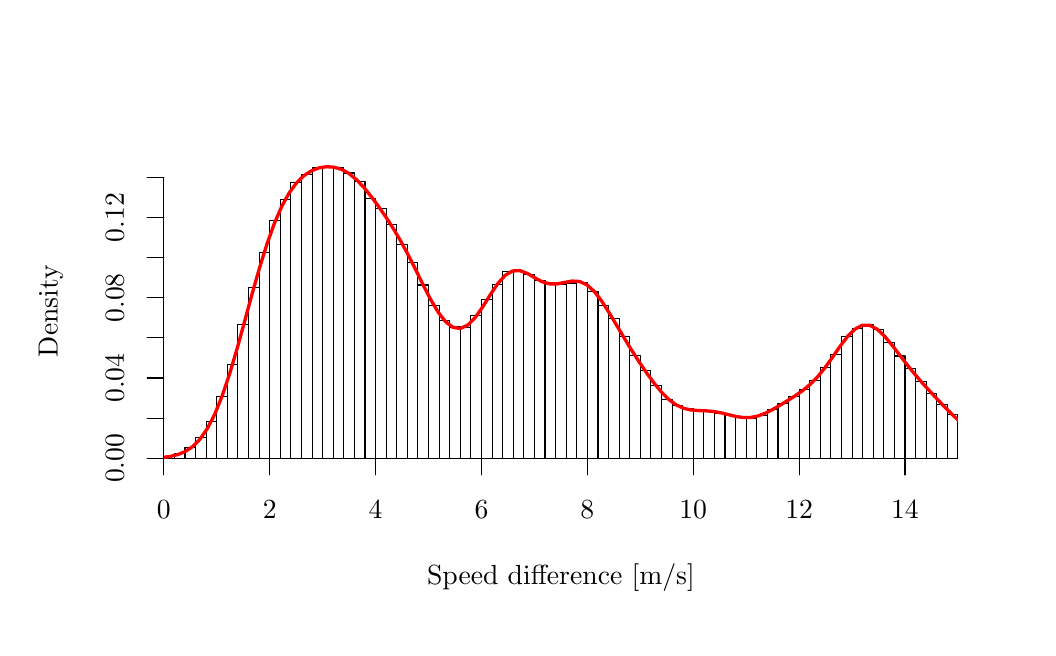
\begin{tikzpicture}[x=1pt,y=1pt]
\definecolor{fillColor}{RGB}{255,255,255}
\path[use as bounding box,fill=fillColor,fill opacity=0.00] (0,0) rectangle (361.35,216.81);
\begin{scope}
\path[clip] (  0.00,  0.00) rectangle (361.35,216.81);
\definecolor{drawColor}{RGB}{0,0,0}

\node[text=drawColor,anchor=base,inner sep=0pt, outer sep=0pt, scale=  1.00] at (192.68, 15.60) {Speed difference [m/s]};

\node[text=drawColor,rotate= 90.00,anchor=base,inner sep=0pt, outer sep=0pt, scale=  1.00] at ( 10.80,114.41) {Density};
\end{scope}
\begin{scope}
\path[clip] (  0.00,  0.00) rectangle (361.35,216.81);
\definecolor{drawColor}{RGB}{0,0,0}

\path[draw=drawColor,line width= 0.4pt,line join=round,line cap=round] ( 49.20, 61.20) -- (317.02, 61.20);

\path[draw=drawColor,line width= 0.4pt,line join=round,line cap=round] ( 49.20, 61.20) -- ( 49.20, 55.20);

\path[draw=drawColor,line width= 0.4pt,line join=round,line cap=round] ( 87.46, 61.20) -- ( 87.46, 55.20);

\path[draw=drawColor,line width= 0.4pt,line join=round,line cap=round] (125.72, 61.20) -- (125.72, 55.20);

\path[draw=drawColor,line width= 0.4pt,line join=round,line cap=round] (163.98, 61.20) -- (163.98, 55.20);

\path[draw=drawColor,line width= 0.4pt,line join=round,line cap=round] (202.24, 61.20) -- (202.24, 55.20);

\path[draw=drawColor,line width= 0.4pt,line join=round,line cap=round] (240.50, 61.20) -- (240.50, 55.20);

\path[draw=drawColor,line width= 0.4pt,line join=round,line cap=round] (278.76, 61.20) -- (278.76, 55.20);

\path[draw=drawColor,line width= 0.4pt,line join=round,line cap=round] (317.02, 61.20) -- (317.02, 55.20);

\node[text=drawColor,anchor=base,inner sep=0pt, outer sep=0pt, scale=  1.00] at ( 49.20, 39.60) {0};

\node[text=drawColor,anchor=base,inner sep=0pt, outer sep=0pt, scale=  1.00] at ( 87.46, 39.60) {2};

\node[text=drawColor,anchor=base,inner sep=0pt, outer sep=0pt, scale=  1.00] at (125.72, 39.60) {4};

\node[text=drawColor,anchor=base,inner sep=0pt, outer sep=0pt, scale=  1.00] at (163.98, 39.60) {6};

\node[text=drawColor,anchor=base,inner sep=0pt, outer sep=0pt, scale=  1.00] at (202.24, 39.60) {8};

\node[text=drawColor,anchor=base,inner sep=0pt, outer sep=0pt, scale=  1.00] at (240.50, 39.60) {10};

\node[text=drawColor,anchor=base,inner sep=0pt, outer sep=0pt, scale=  1.00] at (278.76, 39.60) {12};

\node[text=drawColor,anchor=base,inner sep=0pt, outer sep=0pt, scale=  1.00] at (317.02, 39.60) {14};

\path[draw=drawColor,line width= 0.4pt,line join=round,line cap=round] ( 49.20, 61.20) -- ( 49.20,162.69);

\path[draw=drawColor,line width= 0.4pt,line join=round,line cap=round] ( 49.20, 61.20) -- ( 43.20, 61.20);

\path[draw=drawColor,line width= 0.4pt,line join=round,line cap=round] ( 49.20, 75.70) -- ( 43.20, 75.70);

\path[draw=drawColor,line width= 0.4pt,line join=round,line cap=round] ( 49.20, 90.20) -- ( 43.20, 90.20);

\path[draw=drawColor,line width= 0.4pt,line join=round,line cap=round] ( 49.20,104.70) -- ( 43.20,104.70);

\path[draw=drawColor,line width= 0.4pt,line join=round,line cap=round] ( 49.20,119.19) -- ( 43.20,119.19);

\path[draw=drawColor,line width= 0.4pt,line join=round,line cap=round] ( 49.20,133.69) -- ( 43.20,133.69);

\path[draw=drawColor,line width= 0.4pt,line join=round,line cap=round] ( 49.20,148.19) -- ( 43.20,148.19);

\path[draw=drawColor,line width= 0.4pt,line join=round,line cap=round] ( 49.20,162.69) -- ( 43.20,162.69);

\node[text=drawColor,rotate= 90.00,anchor=base,inner sep=0pt, outer sep=0pt, scale=  1.00] at ( 34.80, 61.20) {0.00};

\node[text=drawColor,rotate= 90.00,anchor=base,inner sep=0pt, outer sep=0pt, scale=  1.00] at ( 34.80, 90.20) {0.04};

\node[text=drawColor,rotate= 90.00,anchor=base,inner sep=0pt, outer sep=0pt, scale=  1.00] at ( 34.80,119.19) {0.08};

\node[text=drawColor,rotate= 90.00,anchor=base,inner sep=0pt, outer sep=0pt, scale=  1.00] at ( 34.80,148.19) {0.12};
\end{scope}
\begin{scope}
\path[clip] ( 49.20, 61.20) rectangle (336.15,167.61);
\definecolor{drawColor}{RGB}{0,0,0}

\path[draw=drawColor,line width= 0.4pt,line join=round,line cap=round] ( 33.90, 61.20) rectangle ( 37.72, 61.20);

\path[draw=drawColor,line width= 0.4pt,line join=round,line cap=round] ( 37.72, 61.20) rectangle ( 41.55, 61.23);

\path[draw=drawColor,line width= 0.4pt,line join=round,line cap=round] ( 41.55, 61.20) rectangle ( 45.37, 61.28);

\path[draw=drawColor,line width= 0.4pt,line join=round,line cap=round] ( 45.37, 61.20) rectangle ( 49.20, 61.48);

\path[draw=drawColor,line width= 0.4pt,line join=round,line cap=round] ( 49.20, 61.20) rectangle ( 53.03, 61.90);

\path[draw=drawColor,line width= 0.4pt,line join=round,line cap=round] ( 53.03, 61.20) rectangle ( 56.85, 62.85);

\path[draw=drawColor,line width= 0.4pt,line join=round,line cap=round] ( 56.85, 61.20) rectangle ( 60.68, 65.04);

\path[draw=drawColor,line width= 0.4pt,line join=round,line cap=round] ( 60.68, 61.20) rectangle ( 64.50, 68.87);

\path[draw=drawColor,line width= 0.4pt,line join=round,line cap=round] ( 64.50, 61.20) rectangle ( 68.33, 74.59);

\path[draw=drawColor,line width= 0.4pt,line join=round,line cap=round] ( 68.33, 61.20) rectangle ( 72.16, 83.60);

\path[draw=drawColor,line width= 0.4pt,line join=round,line cap=round] ( 72.16, 61.20) rectangle ( 75.98, 95.14);

\path[draw=drawColor,line width= 0.4pt,line join=round,line cap=round] ( 75.98, 61.20) rectangle ( 79.81,109.48);

\path[draw=drawColor,line width= 0.4pt,line join=round,line cap=round] ( 79.81, 61.20) rectangle ( 83.63,122.83);

\path[draw=drawColor,line width= 0.4pt,line join=round,line cap=round] ( 83.63, 61.20) rectangle ( 87.46,135.62);

\path[draw=drawColor,line width= 0.4pt,line join=round,line cap=round] ( 87.46, 61.20) rectangle ( 91.29,147.12);

\path[draw=drawColor,line width= 0.4pt,line join=round,line cap=round] ( 91.29, 61.20) rectangle ( 95.11,154.62);

\path[draw=drawColor,line width= 0.4pt,line join=round,line cap=round] ( 95.11, 61.20) rectangle ( 98.94,160.71);

\path[draw=drawColor,line width= 0.4pt,line join=round,line cap=round] ( 98.94, 61.20) rectangle (102.76,163.91);

\path[draw=drawColor,line width= 0.4pt,line join=round,line cap=round] (102.76, 61.20) rectangle (106.59,166.10);

\path[draw=drawColor,line width= 0.4pt,line join=round,line cap=round] (106.59, 61.20) rectangle (110.42,166.66);

\path[draw=drawColor,line width= 0.4pt,line join=round,line cap=round] (110.42, 61.20) rectangle (114.24,166.44);

\path[draw=drawColor,line width= 0.4pt,line join=round,line cap=round] (114.24, 61.20) rectangle (118.07,164.29);

\path[draw=drawColor,line width= 0.4pt,line join=round,line cap=round] (118.07, 61.20) rectangle (121.89,161.12);

\path[draw=drawColor,line width= 0.4pt,line join=round,line cap=round] (121.89, 61.20) rectangle (125.72,155.13);

\path[draw=drawColor,line width= 0.4pt,line join=round,line cap=round] (125.72, 61.20) rectangle (129.55,151.54);

\path[draw=drawColor,line width= 0.4pt,line join=round,line cap=round] (129.55, 61.20) rectangle (133.37,145.65);

\path[draw=drawColor,line width= 0.4pt,line join=round,line cap=round] (133.37, 61.20) rectangle (137.20,138.34);

\path[draw=drawColor,line width= 0.4pt,line join=round,line cap=round] (137.20, 61.20) rectangle (141.02,132.04);

\path[draw=drawColor,line width= 0.4pt,line join=round,line cap=round] (141.02, 61.20) rectangle (144.85,123.83);

\path[draw=drawColor,line width= 0.4pt,line join=round,line cap=round] (144.85, 61.20) rectangle (148.68,116.54);

\path[draw=drawColor,line width= 0.4pt,line join=round,line cap=round] (148.68, 61.20) rectangle (152.50,111.03);

\path[draw=drawColor,line width= 0.4pt,line join=round,line cap=round] (152.50, 61.20) rectangle (156.33,108.66);

\path[draw=drawColor,line width= 0.4pt,line join=round,line cap=round] (156.33, 61.20) rectangle (160.15,108.39);

\path[draw=drawColor,line width= 0.4pt,line join=round,line cap=round] (160.15, 61.20) rectangle (163.98,112.83);

\path[draw=drawColor,line width= 0.4pt,line join=round,line cap=round] (163.98, 61.20) rectangle (167.81,118.43);

\path[draw=drawColor,line width= 0.4pt,line join=round,line cap=round] (167.81, 61.20) rectangle (171.63,123.94);

\path[draw=drawColor,line width= 0.4pt,line join=round,line cap=round] (171.63, 61.20) rectangle (175.46,128.73);

\path[draw=drawColor,line width= 0.4pt,line join=round,line cap=round] (175.46, 61.20) rectangle (179.28,128.80);

\path[draw=drawColor,line width= 0.4pt,line join=round,line cap=round] (179.28, 61.20) rectangle (183.11,127.56);

\path[draw=drawColor,line width= 0.4pt,line join=round,line cap=round] (183.11, 61.20) rectangle (186.94,125.61);

\path[draw=drawColor,line width= 0.4pt,line join=round,line cap=round] (186.94, 61.20) rectangle (190.76,124.71);

\path[draw=drawColor,line width= 0.4pt,line join=round,line cap=round] (190.76, 61.20) rectangle (194.59,124.17);

\path[draw=drawColor,line width= 0.4pt,line join=round,line cap=round] (194.59, 61.20) rectangle (198.41,124.53);

\path[draw=drawColor,line width= 0.4pt,line join=round,line cap=round] (198.41, 61.20) rectangle (202.24,124.64);

\path[draw=drawColor,line width= 0.4pt,line join=round,line cap=round] (202.24, 61.20) rectangle (206.07,121.62);

\path[draw=drawColor,line width= 0.4pt,line join=round,line cap=round] (206.07, 61.20) rectangle (209.89,116.40);

\path[draw=drawColor,line width= 0.4pt,line join=round,line cap=round] (209.89, 61.20) rectangle (213.72,111.71);

\path[draw=drawColor,line width= 0.4pt,line join=round,line cap=round] (213.72, 61.20) rectangle (217.54,105.10);

\path[draw=drawColor,line width= 0.4pt,line join=round,line cap=round] (217.54, 61.20) rectangle (221.37, 98.44);

\path[draw=drawColor,line width= 0.4pt,line join=round,line cap=round] (221.37, 61.20) rectangle (225.20, 92.82);

\path[draw=drawColor,line width= 0.4pt,line join=round,line cap=round] (225.20, 61.20) rectangle (229.02, 87.35);

\path[draw=drawColor,line width= 0.4pt,line join=round,line cap=round] (229.02, 61.20) rectangle (232.85, 82.50);

\path[draw=drawColor,line width= 0.4pt,line join=round,line cap=round] (232.85, 61.20) rectangle (236.67, 80.39);

\path[draw=drawColor,line width= 0.4pt,line join=round,line cap=round] (236.67, 61.20) rectangle (240.50, 79.29);

\path[draw=drawColor,line width= 0.4pt,line join=round,line cap=round] (240.50, 61.20) rectangle (244.33, 78.30);

\path[draw=drawColor,line width= 0.4pt,line join=round,line cap=round] (244.33, 61.20) rectangle (248.15, 78.60);

\path[draw=drawColor,line width= 0.4pt,line join=round,line cap=round] (248.15, 61.20) rectangle (251.98, 77.46);

\path[draw=drawColor,line width= 0.4pt,line join=round,line cap=round] (251.98, 61.20) rectangle (255.80, 76.78);

\path[draw=drawColor,line width= 0.4pt,line join=round,line cap=round] (255.80, 61.20) rectangle (259.63, 76.35);

\path[draw=drawColor,line width= 0.4pt,line join=round,line cap=round] (259.63, 61.20) rectangle (263.46, 75.59);

\path[draw=drawColor,line width= 0.4pt,line join=round,line cap=round] (263.46, 61.20) rectangle (267.28, 76.80);

\path[draw=drawColor,line width= 0.4pt,line join=round,line cap=round] (267.28, 61.20) rectangle (271.11, 78.89);

\path[draw=drawColor,line width= 0.4pt,line join=round,line cap=round] (271.11, 61.20) rectangle (274.93, 80.86);

\path[draw=drawColor,line width= 0.4pt,line join=round,line cap=round] (274.93, 61.20) rectangle (278.76, 83.55);

\path[draw=drawColor,line width= 0.4pt,line join=round,line cap=round] (278.76, 61.20) rectangle (282.59, 86.09);

\path[draw=drawColor,line width= 0.4pt,line join=round,line cap=round] (282.59, 61.20) rectangle (286.41, 89.20);

\path[draw=drawColor,line width= 0.4pt,line join=round,line cap=round] (286.41, 61.20) rectangle (290.24, 93.97);

\path[draw=drawColor,line width= 0.4pt,line join=round,line cap=round] (290.24, 61.20) rectangle (294.06, 98.77);

\path[draw=drawColor,line width= 0.4pt,line join=round,line cap=round] (294.06, 61.20) rectangle (297.89,105.22);

\path[draw=drawColor,line width= 0.4pt,line join=round,line cap=round] (297.89, 61.20) rectangle (301.72,108.14);

\path[draw=drawColor,line width= 0.4pt,line join=round,line cap=round] (301.72, 61.20) rectangle (305.54,109.35);

\path[draw=drawColor,line width= 0.4pt,line join=round,line cap=round] (305.54, 61.20) rectangle (309.37,107.87);

\path[draw=drawColor,line width= 0.4pt,line join=round,line cap=round] (309.37, 61.20) rectangle (313.19,103.06);

\path[draw=drawColor,line width= 0.4pt,line join=round,line cap=round] (313.19, 61.20) rectangle (317.02, 98.18);

\path[draw=drawColor,line width= 0.4pt,line join=round,line cap=round] (317.02, 61.20) rectangle (320.85, 93.53);

\path[draw=drawColor,line width= 0.4pt,line join=round,line cap=round] (320.85, 61.20) rectangle (324.67, 88.85);

\path[draw=drawColor,line width= 0.4pt,line join=round,line cap=round] (324.67, 61.20) rectangle (328.50, 84.71);

\path[draw=drawColor,line width= 0.4pt,line join=round,line cap=round] (328.50, 61.20) rectangle (332.32, 80.77);

\path[draw=drawColor,line width= 0.4pt,line join=round,line cap=round] (332.32, 61.20) rectangle (336.15, 77.16);

\path[draw=drawColor,line width= 0.4pt,line join=round,line cap=round] (336.15, 61.20) rectangle (339.98, 73.30);

\path[draw=drawColor,line width= 0.4pt,line join=round,line cap=round] (339.98, 61.20) rectangle (343.80, 70.50);

\path[draw=drawColor,line width= 0.4pt,line join=round,line cap=round] (343.80, 61.20) rectangle (347.63, 68.07);

\path[draw=drawColor,line width= 0.4pt,line join=round,line cap=round] (347.63, 61.20) rectangle (351.45, 66.19);

\path[draw=drawColor,line width= 0.4pt,line join=round,line cap=round] (351.45, 61.20) rectangle (355.28, 64.93);

\path[draw=drawColor,line width= 0.4pt,line join=round,line cap=round] (355.28, 61.20) rectangle (359.11, 63.93);

\path[draw=drawColor,line width= 0.4pt,line join=round,line cap=round] (359.11, 61.20) rectangle (362.93, 63.16);
\definecolor{drawColor}{RGB}{255,0,0}

\path[draw=drawColor,line width= 1.2pt,line join=round,line cap=round] (  0.00, 61.20) --
	(  0.41, 61.20) --
	(  3.10, 61.20) --
	(  5.79, 61.20) --
	(  8.48, 61.20) --
	( 11.17, 61.20) --
	( 13.86, 61.20) --
	( 16.55, 61.20) --
	( 19.24, 61.20) --
	( 21.93, 61.20) --
	( 24.62, 61.20) --
	( 27.30, 61.20) --
	( 29.99, 61.20) --
	( 32.68, 61.20) --
	( 35.37, 61.20) --
	( 38.06, 61.21) --
	( 40.75, 61.23) --
	( 43.44, 61.26) --
	( 46.13, 61.35) --
	( 48.82, 61.53) --
	( 51.50, 61.88) --
	( 54.19, 62.52) --
	( 56.88, 63.62) --
	( 59.57, 65.40) --
	( 62.26, 68.11) --
	( 64.95, 71.99) --
	( 67.64, 77.22) --
	( 70.33, 83.88) --
	( 73.02, 91.88) --
	( 75.71,100.95) --
	( 78.39,110.68) --
	( 81.08,120.53) --
	( 83.77,129.99) --
	( 86.46,138.62) --
	( 89.15,146.10) --
	( 91.84,152.29) --
	( 94.53,157.16) --
	( 97.22,160.81) --
	( 99.91,163.40) --
	(102.59,165.12) --
	(105.28,166.14) --
	(107.97,166.56) --
	(110.66,166.40) --
	(113.35,165.62) --
	(116.04,164.15) --
	(118.73,161.96) --
	(121.42,159.14) --
	(124.11,155.84) --
	(126.80,152.20) --
	(129.48,148.31) --
	(132.17,144.13) --
	(134.86,139.58) --
	(137.55,134.60) --
	(140.24,129.27) --
	(142.93,123.80) --
	(145.62,118.58) --
	(148.31,114.03) --
	(151.00,110.56) --
	(153.69,108.51) --
	(156.37,108.10) --
	(159.06,109.35) --
	(161.75,112.10) --
	(164.44,115.94) --
	(167.13,120.24) --
	(169.82,124.25) --
	(172.51,127.29) --
	(175.20,128.90) --
	(177.89,129.02) --
	(180.57,127.98) --
	(183.26,126.41) --
	(185.95,124.99) --
	(188.64,124.22) --
	(191.33,124.23) --
	(194.02,124.75) --
	(196.71,125.25) --
	(199.40,125.10) --
	(202.09,123.89) --
	(204.78,121.45) --
	(207.46,117.95) --
	(210.15,113.74) --
	(212.84,109.23) --
	(215.53,104.70) --
	(218.22,100.31) --
	(220.91, 96.11) --
	(223.60, 92.13) --
	(226.29, 88.44) --
	(228.98, 85.16) --
	(231.66, 82.47) --
	(234.35, 80.49) --
	(237.04, 79.26) --
	(239.73, 78.66) --
	(242.42, 78.45) --
	(245.11, 78.35) --
	(247.80, 78.12) --
	(250.49, 77.65) --
	(253.18, 76.99) --
	(255.87, 76.34) --
	(258.55, 75.93) --
	(261.24, 75.96) --
	(263.93, 76.51) --
	(266.62, 77.53) --
	(269.31, 78.90) --
	(272.00, 80.46) --
	(274.69, 82.11) --
	(277.38, 83.82) --
	(280.07, 85.70) --
	(282.76, 87.92) --
	(285.44, 90.65) --
	(288.13, 93.96) --
	(290.82, 97.71) --
	(293.51,101.60) --
	(296.20,105.14) --
	(298.89,107.84) --
	(301.58,109.27) --
	(304.27,109.26) --
	(306.96,107.85) --
	(309.64,105.33) --
	(312.33,102.11) --
	(315.02, 98.60) --
	(317.71, 95.11) --
	(320.40, 91.78) --
	(323.09, 88.65) --
	(325.78, 85.67) --
	(328.47, 82.78) --
	(331.16, 79.96) --
	(333.85, 77.24) --
	(336.53, 74.70) --
	(339.22, 72.40) --
	(341.91, 70.40) --
	(344.60, 68.70) --
	(347.29, 67.30) --
	(349.98, 66.15) --
	(352.67, 65.20) --
	(355.36, 64.42) --
	(358.05, 63.76) --
	(360.73, 63.20) --
	(361.35, 63.09);
\end{scope}
\end{tikzpicture}

	\caption{The histogram shows the result of the conditional sampling according to \cref{alg:constrained hard}. The red line represents the true \ac{pdf}.}
	\label{fig:constrained hard}
\end{figure}
